\documentclass[12pt,a4paper]{book}
\usepackage[left=3cm,right=2.5cm,top=3cm,bottom=2.5cm]{geometry}
\usepackage{eurosym}
\usepackage[utf8]{inputenc}
\usepackage[english]{babel}
\usepackage{amsmath}
\usepackage{amsfonts}
\usepackage{subfigure}
\usepackage{float}
\usepackage{amsthm}
\usepackage{amssymb}
\usepackage{makeidx}
\usepackage{graphicx}
\usepackage{amsmath}              % Matheamtische Formeln
\usepackage{amsfonts}             % Mathematische Zeichensätze
\usepackage{amssymb}  
\usepackage[table]{xcolor}
\usepackage[printonlyused]{acronym}  % Abkürzungsverzeichnis [nur verwendete Abkürzugen]
\usepackage{pdfpages}
\usepackage{appendix}
\usepackage{enumitem}
%\setlist{parsep=0pt,listparindent=\parindent}
\usepackage{float}
\usepackage{titlesec}
\usepackage{fancyhdr}
\usepackage{lastpage}
\usepackage{eso-pic}
\usepackage{caption}
\usepackage{multirow}
\usepackage{multirow, array} 
\usepackage{lmodern}
\usepackage{url}
\usepackage{siunitx}
\urlstyle{rm}
\usepackage[backend=biber,
  isbn=false,                     % ISBN nicht anzeigen, gleiches geht mit nahezu allen anderen Feldern
  %sortlocale=de_DE,               % Sortierung der Einträge für Deutsch
  sortlocale=en_US,              % Sortierung der Einträge für Englisch
  autocite=inline,                % regelt Aussehen für \autocite (inline=\parancite)
  hyperref=true,                  % Hyperlinks für Ziate
  style=ieee                     % Zitate als Zahlen [1]
  %style=alphabetic               % Zitate als Kürzel und Jahr [Ein05]
  %style=authoryear                % Zitate Author und Jahr [Einstein (1905)]
]{biblatex}                      
\usepackage[hidelinks]{hyperref}
\usepackage{subfigure} 
\usepackage{listings}
%\usepackage[justification=centering]{caption}
\setcounter{secnumdepth}{5}
\setcounter{tocdepth}{5}
\makeatletter
\graphicspath{{Imagenes/}}
\usepackage{gensymb}
\definecolor{rojo}{rgb}{0.8,0,0}
\definecolor{verde1}{rgb}{0,0.8,0}
\definecolor{verde2}{rgb}{0,0.7,0}
\definecolor{verde3}{rgb}{0,0.6,0}
\definecolor{verde4}{rgb}{0,0.5,0}
\definecolor{azul1}{rgb}{0,0,0.8}
\definecolor{azul2}{rgb}{0,0,0.7}
\definecolor{azul3}{rgb}{0,0,0.6}
\definecolor{azul4}{rgb}{0,0,0.5}

%TÍTULO Y AUTOR
\author{Jacqueline Franßen}
\title{Development of RFID applications for management and tracking assets and drugs in hospitals}

% formato de cabeceras, con package fancyhdr
\pagestyle{fancy}
\fancypagestyle{bloque_inicial}{%Encabezado y pie de página del bloque inicial con resumen, notación, indices, etc.
\fancyhead{}%limpia todos los campos que se pondrían por defecto
\fancyfoot{}
\cfoot{\thepage}
\pagenumbering{roman}
\renewcommand{\headrulewidth}{0 pt}}

\fancypagestyle{doc_body}{%encabezado y pie de página del bloque del trabajo tal y como están definidos en la plantilla de la EPI
\pagenumbering{arabic}
\fancyhead{}
\lhead{\begin{minipage}{1.8cm}
		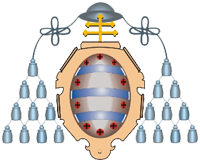
\includegraphics[width=0.8\textwidth]{logo_uniovi.png}
	\end{minipage}
	\begin{minipage}{8cm}
		\scriptsize { 
				\textbf{UNIVERSIDAD DE OVIEDO}}\\
		\footnotesize {
				 \textbf{Escuela Politécnica de Ingeniería de Gijón}}
	\end{minipage}}
\rhead{\footnotesize{\textbf{Hoja \thepage \! \! de \pageref{LastPage}}}}
\fancyfoot{}
\cfoot{\textbf{Jacqueline Franßen}}
\renewcommand{\headrulewidth}{0 pt} %sin línea horizontal en el encabezado
\renewcommand{\footrulewidth}{0.4pt}
}

%% ESPACIADOS
\setlength{\headsep}{20pt}
\setlength{\headheight}{30pt}
\setlength{\footskip}{35pt}
\setlength{\parskip}{12pt}
\titlespacing{\chapter}{0pt}{0pt}{0pt}
\titlespacing{\section}{0pt}{24pt}{0pt} %doble intro antes de inicio de sección, un intro después
\renewcommand{\baselinestretch}{1.5} %interlineado

%Para cambiar la etiqueta Cuadro por Tabla
\addto\captionsspanish{%
\renewcommand{\tablename}{Tabla}}
\addto\captionsspanish{%
\renewcommand\listtablename{Índice de Tablas}}

%Apéndices en castellano
\addto\captionsspanish{%
\renewcommand\appendixname{Apéndice}}
\renewcommand{\appendixtocname}{Apéndices}
\renewcommand{\appendixpagename}{Apéndices}

%%formato del capítulo, apartados y subapartados
\titleformat{\chapter}
{\fontsize{28}{28}\linespread{1}\selectfont\bf}{\thechapter.}{1em}{}

\titleformat{\section}
{\fontsize{14}{14}\linespread{1}\selectfont\bf}{\thesection.-}{1em}{}

\titleformat{\subsection}
{\fontsize{12}{12}\linespread{1}\selectfont\bf}{\thesubsection.-}{1em}{}

\titleformat{\subsubsection}
{\fontsize{12}{12}\linespread{1}\selectfont\bf}{\thesubsubsection.-}{1em}{}

%formato del rótulo de las figuras y las Tablas
\DeclareCaptionLabelSeparator{compuesto}{.- }  %define el nuevo tipo de separador
\captionsetup{labelsep = compuesto} %incluye el separador en el seup de los rótulos de figuras y Tablas

%marca de agua, configuración de su tamaño y posición
\newcommand\BackgroundPic{
\put(70,-40){
\parbox[b][\paperheight]{\paperwidth}{%
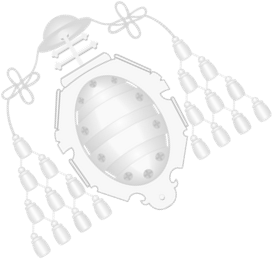
\includegraphics[width=5cm,keepaspectratio]{marca_agua}%
}}}

%cuando te parta una palabra mal entre dos líneas, le indicas aquí cómo quieres que la divida
\hyphenation{e-jem-plo}

%control de líneas viudas y huerfanas
\clubpenalty=10000
\widowpenalty=10000

\pretolerance=2000
\tolerance=3000

\emergencystretch = \maxdimen
\hyphenpenalty = 10000
\hbadness = 10000

\addbibresource{literatur.bib}  

\begin{document}

\pagestyle{bloque_inicial} %utiliza cabeceras definidas en bloque_inicial
\pagenumbering{roman}
%Este bloque va comentado para que no te genere tantas hojas al principio cuando estés escribiendo el documento
%incluye la portada, y los bloques de agradecimientos, resumen, acrónimos y notación (yo incluiría resumen y notación/acrónimos mínimo)


\includepdf{portadaInterior}
\cleardoublepage
\cleardoublepage
%a continuación el índice (general, de figuras y de Tablas)
\addcontentsline{toc}{section}{\textsc{Contents}}
\tableofcontents
\cleardoublepage
\addcontentsline{toc}{section}{\textsc{List of figures}}
\listoffigures
\cleardoublepage
\addcontentsline{toc}{section}{\textsc{List of tables}}
\listoftables

%%%%%%%%%%%%%%%%%%%%%%%%%%%%%%%%%%%%%%%%%%%%%%%%%%%%%%%%%%%%%%%%%%%%%%%%%%%%%%%%%%%%%%%%%%%%%%%%%%%%%%%%%%%%%%%%%%%%%%%%%%%%%%%%%%%%%%%%%%%%%%%%%%%%%%%%%%%%
% 						CUERPO DEL TFG
%%%%%%%%%%%%%%%%%%%%%%%%%%%%%%%%%%%%%%%%%%%%%%%%%%%%%%%%%%%%%%%%%%%%%%%%%%%%%%%%%%%%%%%%%%%%%%%%%%%%%%%%%%%%%%%%%%%%%%%%%%%%%%%%%%%%%%%%%%%%%%%%%%%%%%%%%%%%%
\newtheorem{mydef}{Definition}
\newpage{} % los capítulos empiezan en página nueva
\pagestyle{doc_body} % para usar los encabezados y pies de página definidos para el cuerpo del documento
\pagenumbering{arabic} 
%\AddToShipoutPicture{\BackgroundPic}% añade la marca de agua

\chapter{\textbf{Introduction}}
The following Bachelor Thesis describes the development of a mobile hybrid application which can be run both on Android and iOS devices as well as the physical layer hardware based on RFID technology. The developed system (both hardware and software) is devoted to be used for tracking and management of medical assets and drugs in hospitals. Compared to other existing systems, the given thesis includes the development of 'real-time' synchronization between client and server, realized by Socket.IO. Thus, a very synchronous solution approach is pursued in order to react contemporarily to missing drugs.

The project aims to develop a RFID-based system for management and tracking applications. In particular, the proposed system is devoted to be deployed at hospitals, to ensure a better control of the medicines and medical tools that are periodically administered to the patients, reducing the probability of missed or wrong medicine administration. The proposed system is formed by a set of RFID antennas that will conform the coverage area where items tagged with RFID tags will be read. These antennas and the RFID reader will be connected to a database that will contain the information of the items to be monitored. The project covers topics of great interest for medical and \ac{ITC} companies, such as IoT and e-Health.

\chapter{Use, Scope and Limitations of RFID Technology}
\label{Kap1}

The following chapter will discuss the reasons why to choose the RFID technology. In the beginning, in the 'Motivation' section there will be described some state of the art applications. After that, the section 'Aim and Scope' will introduce the limits of the RFID technology and of its applications which should be considered during the deployment. In the end, there will be outlined the \ac{SWOT} method to analyze the benefits and threats of an RFID application.

\section{Motivation}

Concerning the organization and management of medical devices or patients in a hospital, there exist many problems. In the following, some solutions to these problems, as described by Ajami and Rajabzadeh \cite{ncbi}, will be depicted.

\subsection{Decision Making}

First of all, when it comes to decision making, e.g. about the correct treatment of a severe illness, many physicians are stumped for an answer or their opinions are divided. To enable a rapid diagnosis and to improve the patient's health status, 'smart healthcare' \cite{henrici} would help a lot. 'Smart healthcare' includes RFID tags which are equipped with sensors to ensure the effectiveness of a medical treatment. This accelerates the treatment process a lot. Furthermore, patients or hospital beds equipped with RFID tags make it easier to identify and manage the amount of patients as well as the workflow.

\subsection{Internal Communication}

Secondly, poor communication between nurses and physicians deteriorates medical supply. For instance, if a nurse notices that a patient needs more tranquilizer because he became very nervous, she has to tell the doctor to dose the patient with the correct amount. But often, a physician is occupying another patient. So, there exists the problem of communication and further the staff shortage in many healthcare institutions. Thus, inadequate patient monitoring emerges. It should be added that sometimes, there is the risk of misidentification of patients. To explain the last point, one should think of this easy example: At the urology department are two elder patients, Paul Schmitt and Jochen Schmitt. They are not brothers or related to each other and suffer from different types of illness. Paul suffers from kidney insufficiency whereas Jochen suffers from prostatic lithiasis. The first one needs a dialysis every day whereas the second one needs a radiosurgery. Because both patients are unable to walk themselves, nurses and clinical staff have to bring them to the particular treatment room. The problem should be easy to understand, both patients have the same surname but need completely different treatments. If the treatments would be commuted, their health status would deteriorate and they might die because of the misidentification.

\subsection{Production process}

To give another example of the successful deployment of  RFID solutions, Tamm and Tribowski \cite[p.110 ff.]{fokus} outline the company 'Gerry Weber'. In the following, some benefits of the RFID application will be explained. Firstly, count and identification processes of goods could be accelerated by using the RFID technology. Secondly, both the electronic article surveillance and RFID minimize costs and time. Thirdly, the delivery quality was improved and mistakes were reduced and sometimes avoided. Fourthly, the logistic was improved by the improved transparency of stock. Fifthly, the existing heterogeneous systems can be controlled more easily. Lastly, there might occur some reading processes without focus which means that the adjacent items are reflected and erroneously detected. This can be avoided by filtering involuntary readings via software filters.  

\subsection{Investment possibilities}

Another important point for hospitals is the budget and their possibilities to investigate in new technologies which makes the enrollment of a new RFID system more challenging. Furthermore, clinical staff and phycisians have to be introduced into the new technologies. Not only the human factor plays a significant role but also the existing systems, such as the \ac{HIS}, \ac{RIS} or \ac{LIS}. If a new identifying system or software shal be integrated into a hospital or healthcare institution, it has to be deployed suitably to the existing system architecture. To achieve the last point, Ajami and Rajabzadeh \cite{ncbi} recommend starting with small RFID projects and mention countermeasures to increase the acceptance of such applications by healthcare institutions. To give an example, the regulations to protect patient's privacy should be mature to achieve more institutional support. Besides, there should exist more customized RFID systems which accomplish the individual tasks of their users.  

\subsection{Medication Administration System}

To explain the positive impact of using RFID systems, in the following, a few applications will be described briefly (see also \cite{ncbi}). Firstly, Ajami and Rajabzadeh describe a Medication Administration System which automatically verifies medication and generates the corresponding prescription. There exist multiple intents of developing an Administration System, such as preventing human errors (like for example mislabeling of tissue specimens in gastrointestinal and colorectal surgery endoscopy units). The second most common error which occured were that patients have been labelled incorrectly. To avoid these errors, an initiative of developing an RFID application to specimen bottles was started. The aim of this initiative was to create a paperless pathology requisition system which correctly confirms boths the endoscopy nursing staff as well as the endoscopist for each specimen bottle. After deploying the application, specimen-labeling errors were significantly reduced.

\subsection{Wisely Aware RFID Dosage}

Another RFID system, called \ac{WARD} system should prevent the risk of medication errors triggered by medical staff. It is based on an integrated barcode and RFID tags which should demonstrate effective and safe patient care environment. 
Not only the correct dosage can be controlled by RFID but also medical staff. The following paragraph will describe the \ac{MIMS} which includes a mobile nursing care system using RFID technology. There are many implemented functionalities in the MIMS, such as the tracking of patient's vital signs across various locations and in different medical facilities. The vital sign monitoring enables medical staff to watch critical ill patients carefully and permanently and reduces the risk of serious harm resulting from slow provision \cite{ncbi}. Moreover, it offers alarming services in case of emergencies and can always be taken everywhere. Behind the frontend, a rule-based clinical decision supports medical staff and the mobile nursing environment. Last but not least, MIMS has been extended to most medical domains and has been integrated into other HIS.

\subsection{RFID applications in hospitals: A case study}

In their conference paper, Wang et al. \cite{casestudy} describe a case study of implementing a RFID system in a Taiwan hospital in the year 2003. The project was named \ac{LBMS} and performed at the \ac{TMUH}. In the following section, the development strategy, device management as well as the value generation which were important for developing the LBMS will be explained. 
Referring to a widely spread disease, called \ac{SARS} in 2003, the authors Wang et al. discuss the effectiveness of applying RFID in hospitals to prevent further infections (e.g. of patients or medical staff). They mention several challenges of implementing RFID systems in hospitals, for instance user or physician resistance, investment problems as well as technical, clinical, organizational and professional resistance. Nevertheless, some hospitals initiated (with subsidies from the Taiwanese government) preliminary RFID projects as early as October 2003 and achieved significant results. 

To give a basic introduction into the existing IT infrastructure at the TMUH, the following paragraph will mention the existing systems of the hospital. TMUH has an integrated HIS that complies with several healthcare standards, such as \ac{HL7}, \ac{DICOM} \cite[p.3 ff.]{casestudy}. Furthermore, the system consists of a LIS, RIS and according to Wang et al. most of the patient's medical records are digitalized. When it comes to the development and the reasons for using LBMS, the authors claim to build a system that could detect and track potential SARS cases. Besides, medical knowledge and practice should form the basis and core for developing the system. The RFID technology was considered as a tool to support medical practice. In the end, the system should reflect medical assumptions. 
Wang et al. describe a basic workflow with four steps of the LBMS: Initially, all data should be stored in a positioning database which is connected to the existing vital information databases (of the HIS). In the second step, the system automatically retrieves patient medical records from the HIS and runs an inference engine (called 'Rulebase').  'Rulebase' judges whether there was an infectious event or not. If there was a infectious event, the system detects this in a third step. As a consequence (step four) of the detected event, a message is sent immediately to the relevant personnel through an alarm (email and sms). 
The LBMS can be extended and used in other contexts, like e.g. for precious equipment tracing, in-patient medicine auditing, new-born baby and mother identification or to legitimate drug control.
Wang et al. were supported by the Taiwanese government which approved their plan and granted money. Since the LBMS should be released as a hospital-wide system, the development required expertise and knowledge from different domains, including medicine, RFID technology, IT systems development, telecommunications and systems integration. Actually, three parties were involved: TMUH, Lion Information Inc. and an advisory group \cite[p.4]{casestudy} which consisted of professors who emerged the technology and made academic contributions (algorithms).
Since the hospital decided that the system should have active real-time position-tracking, temperature taking and monitoring abilities for tagged patients, the developing team chose 916,5 MHz UHF active tags (see Chapter 2, RFID tags \pageref{tag}) to reduce the risk of staff infections.

Reaching an adequate system integration without loss of performance, functionality and security was a big challenge. With the use of a field generator, a small tag wake-up device that communicates directly with the reader, the real-time communication should be realized \cite[p.4]{casestudy}. The generator periodically turns on and calls tags for a specific time. There exist three different types of generators: Normal, floor and area generators.
Furthermore, Wang et al. bring up the challenge of the entire device management \cite[p.5]{casestudy} with the purpose of collecting and transmitting reads that are as complete and clean as possible. Realizing a complete device management was limited by compartments, rooms, walls and doors because of their buildling layouts and materials which interfere with radiowaves. Besides, the balance between accuracy requirements and investment costs has to be maintained. Moreover, unauthorized removal of tags has to be managed carefully, since there might be some patients who try to take off their RFID wristband. In this case, an additional alarm has to be designed. Basically, the design and deployment of RFID devices depend on the environment and the context in which they are used. 
Not only the device management was challenging but also the data management as Wang et al. mention. The authors describe two general problems of data management in their RFID system. On the one hand, there will occur intermittent and unreliable reads. These can be compensated by developing algorithms to process missing and incomplete reads. On the other hand, there will be generated high-volume data in a very short time. To prohibit this, the data should be filtered by algorithms and only the necessary data should be transmitted. For instance, if a tagged patient exceeded the present degree of 0.5\celsius, his data would be transmitted. To come to a conclusion, data management is tied to medical knowledge and practices which can substantially reduce the volume of data to be handled. As a result, meaningful information for decision making will be generated.
 
Besides the LBMS project \cite[p.2 ff.]{casestudy}, Wang et al. depict some existing RFID applications. To give an example of a successful use of RFID, the U.S. Department of Defence has been using the technology for years. 
To give an overview of the usual hospital applications until 2006, Wang et al. describe applications for tracking and managing equipment such as wheelchairs or portable heart monitors. Moreover, trials on tagging patients, staff and equipment in rooms were conducted in several hospitals. Besides, the Washington Hospital Center (Washington D.C.) deployed a RFID system to track the status and the exact location of patients, staff as well as the essential equipment.
During the realization of the mentioned projects, the solutions depended on building an RFID infrastructure together with the middleware and the impedance-matching of the RFID system and the current systems (e.g. \ac{ERP} systems). Actually, to get along with the mentioned solutions, a strong team work (involving people from IT and business departments) and project management should be included. 
Since RFID allows wireless storage and automatic retrieval of data, there exists an 'ecosystem' of companies trying to develop a platform to support RFID development and applications.  Besides, the variety of existing systems in hospitals, Wang et al. mention three mayor technical challenges accomplishing a RFID system. First, the non-line-of-sight reading might be a challenge since there exist various types of tags and the frequencies influence the range of signal. Second, handling the serial numbers can be difficult but it could be coped with setting a primary key to each tag which synchronizes with an existing database (see Chapter 3, 'Used platforms and technologies' \pageref{platforms}). The third challenge is to deal with the real-time data and to synchronize these seasonably. To deal with that, the use of NoSQL databases makes sense and will be discussed in Chapter 3 \pageref{nosql}.

Finally, Wang et al. evaluate RFID as an infrastructure technology which allows companies to capture data about objects and individuals moving in the real world \cite[p.7]{casestudy}. In addition to that, the authors recommend that organizations should think carefully how to change business processes to reap the benefits of RFID. By naming benefits of RFID, Wang et al. refer to the improved efficiency, patient safety and reduced medical errors which can be very extensive and expensive nowadays \cite{casestudy}.

\section{Aim and Scope}

Ajami and Rajabzadeh \cite{ncbi} mention three important purposes of RFID technology. The first purpose of using RFID is to improve the tracking of objects. It is mainly used to follow products through a specific supply chain or to follow medical devices an drugs in the clinical workflow. There is also the possibility to track a product to a particular patient or to identify clinicians who administered medication to patients.
The second purpose for which RFID technology is appropriate is the inventory management (see section \pageref{inventory}). Inventory Management is significant for managing items of an organization, like a hospital. There are many complex processes where information about the location, time and the amount of material is necessary (e.g. towels, duvet covers).
The third and last purpose of RFID technology, mentioned by Ajami and Rajabzadeh \cite{ncbi}, is validation. Using RFID to identify and validate data is an effective method for ensuring the quality of a hospital or healthcare setting. It ensures that the patient being treated is the right patient.

\subsection{RFID and the IoT}

There exist many applications, which should help us living smarter, not caring about the ordinary things, like for example turning off the washing machine or closing the windows before stepping out. These smart houses form a part of the term \ac{IoT}. Often, the smart solutions are based on RFID technology to identify the exact window or the item that has to be controlled from outside. 
In their book 'RFID Technologies for the Internet of Things', Chen et al. \cite[p.2 f.]{chen} depict smart applications and a specific difficulty which they call the 'Tag Search Problem'. It usually appears on large-scale RFID systems and describes the complexity of identifying the wanted tags which exist in the current system. To solve this identification problem, Chen et al. describe the method 'Filtering vectors' which will be explained in the following. 
Firstly, a compact one-dimension bit array is constructed from the tag IDs which are used for filtering the unwanted tags. After that, a novel iterative tag search protocol is run. This protocol progressively improves the accuracy of search results and reduces the time by using information which were detected from previous iterations.
As a second problem of IoT applications, Chen et al. mention the conflict with people's privacy \cite[p.3 f.]{chen}. Since every tag transmits its ID to the nearest reader, the transmission can be exploited by attackers. To prevent eavesdropping, the authors describe an anonymous RFID authentication mechanism which designs anonymous authentication protocols. The protocol is based on cryptographic hash functions which require considerable hardware to randomize the authentication data in order to make the tags untrackable. At this point, one should keep in mind that the provided solution requires valuable hardware and is not suited for low-cost tags which augments the production costs. Thus, manufacturers have to face the challenge of designing anonymous authentication protocols for low-cost tags given their limited hardware resources. 
To face the problem of limited hardware resources, Chen et al. suggest an 'asymmetric design principle' \cite[p.4]{chen} which means pushing most of the system's complexity to the reader and leaving the tags as simple as possible. 
Besides the anonymous RFID authentication, tags can be identified by their network \cite[p.4 f.]{chen}. To give an example, in large warehouses there exists a great number of readers and antennas which must be deployed to provide full coverage. To accomplish the full coverage, networked  tags which relay transmissions towards the otherwise-inaccessible reader can be used. As a characteristic of networked RFID tags, they are powered by batteries and rechargeable energy sources (harvest solar, piezoelectric, thermal energy from surrounding environment).
Generally, there can be distinguished two types of ID collection protocols: On the one hand, there is the contention-based ID collection protocol which creates too much overhead in multihop networked tag systems. This leads to an increased collision in the network towards the reader and causes excessive energy costs. On the other hand, Chen et al. mention a serialized ID collection protocol. This solution is based on serial numbers that balance the load and reduce worst-case energy costs. 
As a conclusion, one can say, that imbalanced load in a network leads to worst-case energy costs which should be avoided.

\subsubsection{Compact Approximator based Tag Searching protocol}

To avoid the above mentioned energy costs, resulting from inefficient protocols, Chen et al. describe several tag searching protocols \cite[p.13 ff.]{chen} which will be discussed in the following. 
To begin with, one should keep in mind the method 'Filtering vectors' mentioned at the very beginning of this paragraph in which the tag ID was converted into a one-dimension bit array. This first step can be compared with the first step of \ac{CATS}, a two-phased protocol to address the tag identification and its polling problem. The idea of CATS is to encode the tag IDs into a 'Bloom' filter \footnote{A Bloom filter is a compact data structure that encodes membership for a set of items $S=\{ e_{1},e_{2},e_{3},...,e_{n}\}$. To represent S, a bit array of length l is needed. At the beginning, all bits are initialized to zeros. To encode each element $e \in S$, k hash functions are used to map the element randomly to k bits in a bit array, so that the zeros turn into ones.} \cite[p.15]{chen} and to transmit the Bloom filter instead of the ID. 
Consequently, in the first phase of CATS, the RFID reader encodes all IDs of the wanted tags into a Bloom filter. After encoding, the reader broadcasts the filter together with some parameters to the tags in the coverage area. Each tag receives its Bloom filter and tests whether it belongs to set X. Unwanted tags will be kept silently for the remaining time. Furthermore, a second set Y defines the coverage area of the RFID system. After filtration, the number of candidate tags in Y is reduced.
The second phase of CATS deals with the remaining candidate tags from phase 1. These tags report their particular Bloom filter during several time slots. Each candidate tag transmits in k slots and is mapped to a certain set. During the transmission, the reader is listening to the channel and builds a second Bloom filter based on the status of time slots: '1' stands for a busy slot which means that at least one tag is transmitting whereas '0' stands for an idle slot during which no tag is transmitting. 
These two phases build the main activities of the CATS protocol and seem to be realized very easily. Nevertheless, Chen et al. introduce some raising problems by using CATS. One problem is optimizing the Bloom filter sizes since CATS approximates two Bloom filters together as the first, so that $|X \cap Y|=|X|$. A second problem is that CATS assumes that the first Bloom filter is always smaller than the second one: $|X|<|Y|$. But in reality, the number of wanted tags may be far greater than the number in the coverage area of the RFID system. 

\subsubsection{Iterative Tag Search Protocol}

To avoid the errors caused by using CATS, Chen et al. describe another effective tag search protocol which is called \ac{ITSP} \cite[p.22-28]{chen}. Assuming that there is a wireless channel available between the RFID reader and the tag, ITSP interferes from nearby equipment (e.g. motors, conveyers, robots, WLANs, cordless phones). Furthermore, ITSP divides the bidirectional filtration of the tag search process into multiple rounds. Before each round i, a set of candidate tags in X is denoted as $X_{i}(\subseteq X)$ which represents the search result after $(i-1)$ round. Thus, the final search result is a set of remaining candidate tags in X after all rounds are completed. So, ITSP can be seen as a general iterative approach allowing multiple filtering vectors to be sent consecutively. Each round contains two phases. During the first phase, the RFID reader constructs $m_{i}$ filtering vectors for $X_{i}$ using $m_{i}$ hash functions \cite[p.22]{chen}. In a second step, the reader broadcasts the filtering vectors one by one and each tag receives its own filtering vector. By checkiing its ID with the filtering vector, each tag uses the same hash function as the reader. As a result, each tag can get a '1' which means that is it a candidate tag of $Y_{i+1}$  or it receives a '0' which excludes the tag and drops it out of the search process.

Afterwards, during the second round, the reader broadcasts the frame size $L_{Y_{i+1}}$ to the tags (which are all candidate tags) and each tag does the same as in round one. After receiving its filtering vector, each tag randomly maps its ID to a slot in the time frame using a hash function and transmits a response to the reader $(0 or 1)$. After receiving the response from each tag, the reader constructs a new filtering vector which is used to filter the non-candidate tags from $X_{i}$.

After the two phases the reader updates the current stage which contains a set of remaining candidate tags. The number of tags shrinks from $X_{i}$ to $X_{i+1}$ during this step. 

\subsubsection{Lightweight Anonymous RFID Authentication}

There exist many different authentication mechanisms in RFID applications. To give an example of one current possibility to authenticate RFID tags, Chen et al. depict the 'Lightweight Anonymous RFID Authentication' \cite[p.39 ff.]{chen}. To start with, a fundamental system model is given (see figure~\ref{fig:lightweight}). In addition to the system model, it should be noticed that each tag is pre-installed with some keys for authentication. Furthermore, all readers are deployed at chosen locations and connected to backend servers which are connected to a central server. On the central server, each tag's key is stored.

\begin{figure}
\centering
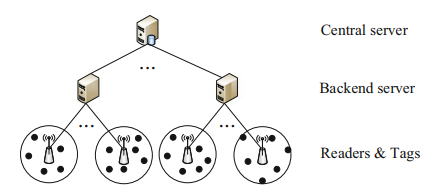
\includegraphics[width=\textwidth]{leightweight} 
\caption{\label{fig:lightweight} The system model of Lightweight Anonymous RFID Authentication \cite[p.40]{chen}} 
\end{figure}

Concerning the communication between readers and tags, Chen et al. describe a 'Request-Response mode Communication' \cite[p.40 ff.]{chen}. Firstly, the reader initiates the communication with the tag by sending a request to it. Secondly, after receiving the request, the tag makes an appropriate transmission as response. There can be distinguished two types of transmissions: Invariant and variant transmissions. The first type (invariant transmissions) can contain content that is 'invariant' between the tag and the reader. In contrast to that, variant transmissions can contain content that may vary for different tags or the same tag at different times, e.g. the exchanged data for anonymous authentication.  

\subsubsection{Identifying state-free networked tags}

Before explaining the mechanism of identifying state-free networked tags, the two terms 'state-free' and 'stateful' networked tags should be made clear. If a networked tag is called stateful, it maintains its networks state which includes information about its neighbors in the network, routing tables as well as update information. In contrast to that, state-free tags serve the purpose of energy conservation and do not maintain any network state prior to their operations which differs them from traditional networks. 
Given the two definitions, there comes up the challenge of identifying state-free networked tags. Chen et al. refer to that challenge and explain a method for identifying networked tags \cite[p.67 ff.]{chen} which will be discussed in the following. 
First of all, all tags in a network are connected to each other through a peer communication (to the nearby tags). Especially the emerging number of networked tags represents a significant enhancement to today's RFID technology. The problem of readers which cannot cover all tags due to cost or physical limitations can be solved by using networked tags. Moreover, the possibility of peer communication enables a multihop network to be formed among the tags. The transmission range of inter-tag communications is usually short and amounts to about 1-10 m whereas the transmission range of a reader is much larger. 
Nevertheless, the peer communication realizes a direct two-way communication between the current node and the neighboring node. Concerning the energy input, the energy can be powered through the reader's radio waves but the internal energy should be carried sufficiently for long-term operations (must be made energy-efficient).
After establishing a peer-to-peer communication, the reader collects the IDs from all networked tags that are in its read range. Using multiple hops and intermediate tags relaying the IDs of those tags which are not in the immediate coverage area of the reader, state-free tags can be identified. 

\subsection{RFID and Mobile Computing}

Concerning the development of mobile applications in context of the RFID technology, the following paragraph discusses fundamental definitions of mobile computing as well as general architecture patterns, like e.g. \ac{SOA}. 
To start with, Hanhart declares in his book \cite[p.9 ff.]{mobile} the term 'mobile computing' as following: '[...] all processes, activities, applications in a company which are proceed by mobile technologies. The company's staff gets access to data and applications (independently from location and time). The focus is set on man-machine-communication [...]' \cite[p.9 ff.]{mobile}. 
When it comes to mobile applications which are connected to RFID systems, Hanhart mentions the term of 'Smart things' or 'Embedded systems' which include physical objects, extended by the RFID sensor technology and which are networked to each other. To achieve some understanding among all readers, Hanhart depicts three types of wireless communications technology \cite[p.12-13]{mobile}. Firstly, there exist mobile communications which consist of a service provider and several mobile devices. The service provider transmits the speech and data from and to mobile devices through a wireless network. 
Secondly, Hanhart notices \ac{WLAN} which enables accessing to a company's network. To give an example, there exist many WLAN hotspots in hotels and airports, which can be accessed simply. Thirdly, there exist 'wireless personal networks' which connect terminal devices with peripheral devices within small ranges. For instance, Bluetooth or \ac{IrDA} are used to transfer data over small distances. Not only Bluetooth and infrared light are used to transfer data, but also ZigBees and \ac{NFC} is used in many cases \cite[p.12-13]{mobile}. Hanhart describes NFC as a newer technology which consists of an active and passive unit. Actually, NFC is only used for connections of a few centimeters, e.g. in consumer electronics. The active unit can be kept in the mobile because it is very small and the data rate amounts to at least 424 kbit/s.
 
\subsubsection{Basis functions of mobile computing and RFID}

When it comes to the use of mobile applications and RFID, one can distinguish between five general scenarios \cite[p.13 ff.]{mobile}. First of all, since RFID enables wireless connection and detection of several items in our environment, it can be used to access mobile applications through the RFID signal. For example, staff can use mobile devices to access (via RFID) business applications and to implement transactions. Secondly, as already mentioned in further sections above, RFID has the main purpose of identifying objects. In combination with mobile devices, there can be established applications which can both identify users and objects. As a third scenario, mobile RFID applications the capture of statal and environmental data. By using sensors, the continuous capture of data is possible. Moreover, smart objects and mobile devices can transform the information directly into actions or convey the data to a central system (or database). As a fourth scenario for using RFID in the context of mobile computing, Hanhart \cite[p.13 ff.]{mobile} remarks the possibility to locate precisely objects and users. Besides, the detected positions can be used to display contextual information or to direct to procedures in backend systems. Last but not least, the purpose of sending notifications in time, can improve and prevent several emergency situations (e.g. in a hospital). Since objects can send notifications e.g. when reaching a certain state, users get information everytime and everywhere.  

\subsubsection{Constraints of mobile applications and RFID}

Developing mobile applications with the RFID technology not only brings advantages, but also challenges when facing for example the user's needs and requirements. Hanhart indicates some 'constraints' of mobile applications and RFID \cite[p.16 ff.]{mobile} which will be depicted in the following. Firstly, the user interface should be considered. In case of healthcare applications which can be used by nurses, staff and physicians there should exist various user roles and rights. Thus, each user needs his specific interface and only a few (or one single) users are able to see all information of a patient. As a further matter, the mobile application should meet the requirements of connecting quality and service quality. This indicates the exact adaption of a service, specified in the requirements specification document. By the same, the challenge of computing capacity in the developer team should be attended. Furthermore, both principal and agent should be aware of the needed development time to realize all required features (which depends on the size and skill level of the developers). In addition, the technical resources, like e.g. memory capacity and energy supply represent another challenging factor. To deal with the last mentioned challenges, it should be favourable to have some sponsors which can support the project.

\subsubsection{Service-oriented architectures}

To cope with the constraints and challenges during the development of a mobile RFID application, Hanhart describes \ac{SOA} \cite[p.31 ff.]{mobile}. SOA is a multilayered, distributed information system architecture which encapsulates parts of an application into business-like services, considering design principles to enable a simplified process integration \cite[p.32]{mobile}. A service can be seen as an abstract software element or interface which provides standardized access to application functions of other applications through a network \cite[p.32]{mobile}. There exist four general design principles with respect to the development of SOA applications. The first design principle is called 'Orientation of Interfaces' which means that the service interfaces abstract implementation from the user's view. What is more, each service has a stable interface which is technically and functionally defined by its metadata. The second design principle of SOA is 'Interoperability' which can be assured by implementing technical and functional standards. This enables the interoperability of a services and its usage in different contexts. The third design principle is called 'Autonomy and Modularity' which signifies that SOA restructures the applications architecture into autonomous subsystems (domains and services). The aim is to increase cohesion in one system and to minimize the linkage between its subsystems. The fourth design principle of SOA is 'Orientation of needs'. This implies that all services should be oriented towards business objects and process activities in order to provide an approximately granular, functional definable output. 

\paragraph{Domain Architecture}

The Domain Architecture is a conceptional foundation of SOA. It reveals duplicates in an existing application architecture. Moreover, it is a fundamental decision foundation for service characteristics. Last but not least, it gives a list of possible service candidates which support systematic integration, development and usage of services.

\subsubsection{Service-oriented proposal of architecture}

In the previous section, the general characteristics of SOA have been discussed. But in which context SOA applications are regularily used? And how is SOA realized? To give answers to these questions, in the following the purpose and integration procedure of SOA applications will be explained. 
First of all, the conditions and prerequisites for an economic realization of diverse solutions based on mobile computing and RFID are simple and flexible integration into existing system architectures \cite[p.133 ff.]{mobile}. The classical integration of mobile terminal devices involves different middleware components and functions which can have different varieties of architecture (with advantages and disadvantages). Modern application systems are multilayered, for example 3-tier/n-tier-architectures. The three tiers include the client (implemented software-components), middleware (necessary components to connect client and backend) and backend (business data and functions) tier. The term 'mobile middleware' refers to the extension of the classical client-server architecture with the aim of improved scalability and administration.
Not only a mobile middleware is needed for an appropriate integration into SOA, but also a RFID middleware is needed. The following paragraph will mention some functional requirements to this specific middleware. First of all, transformation functions are needed to convert RFID raw data into useful business process data. This includes filtering of errors as well as harmonizing the data formats of different device manufacturers. Secondly, there are configuration functions needed for monitoring and controlling the RFID infrastructure. As follows, a configuration function is able to identify readers, manage configuration data, monitor device functionality and ensure security.  

\paragraph{Classic Integration Mechanism}

As a third type of integration, concerning mobile computing and RFID, the integration of embedded devices should be considered. Basically, there are three different tiers: Field tier, Automation tier and Management tier. The first tier, Field tier includes the physical connection of sensors, actuators and control units. The second tier, Automation tier, consists of control units which undertake automatic monitoring and processing functions, like for instance the control of temperature. The communication units connect the control units, programming units and the management tier. The third tier, called Management tier, subsists of monitor and control systems and visualizes them to the operator. Additionally, the Management tier delivers software responsive over proprietary interfaces and can be seen as data handling unit. 
To conclude, the Automation tier can be seen as the communication unit and middleware between Field tier and Management tier. Further, Automation and Management tier can connect to third-party-applications via data interface units.
 
\paragraph{Modern Integration Mechanism}

The last paragraph dealed with integration mechanisms on the real old way. Recently, there are newer technologies and possibilities to realize an integration, such as web services and the emerging communication protocol \ac{SOAP}. In context of web technologies and services, there comes up the term \ac{ESB} \cite[p.141 ff.]{mobile} which provides a standardized interface and communication layer. An ESB is a consistent integration architecture which defines standards as well as central services and provides them for software development, publication and usage. Regarding the integration of mobile applications, the ESB \cite[p.143]{mobile}, there are differentiated two types of integration scenarios: a) the mobile client calls directly the provided services from application domains or b) the client keeps communicating with the services via its mobile middleware. If the client wants to call a service directly, he has to implement its \ac{API}. Besides, for service call or invocation, the standardized interface technology has to be used.
In the matter of integration of RFID systems and embedded devices, the middleware of RFID systems uses the provided services of the application domains, provided by the ESB. In addition to that, mobile applications can be integrated both online and offline \cite[p.146 ff.]{mobile}. Hanhart is using the term 'online' in context of saying that the mobile device runs the user interface. This indicates that the mobile middleware prepares contents of application (for prompt). After that, the application accesses the backend or invoked app through a service which uses the application's functionality via services. In contrast to that, Hanhart uses the expression 'offline' in order to say that the application is running on the client. Here, the mobile application acts as an invoked application and synchronizes its data through the mobile middleware with the backend. The central management of process states (on the client) and synchronization with services are realized through the middleware directly.

\paragraph{Capabilities of SOA, mobile applications and RFID}

To explain the capabilities of the above discussed technologies and architecture, Hanhart brings up 'Reuse', 'Isolation of Domains' and 'Easy implementation'. Reuse is generated by consistent functionalities of interfaces. Isolation of domains is produced by separation of concerns and core data concepts. Easy implementation refers to cross-domain workflows or taskflows. Concerning possible usage scenarios, Hanhart mentions some examples \cite[p.207 ff.]{mobile}, like event-driven process management which includes the automatic capture of events. Or, if it comes to the control of several processes and activities in a company, these activities can be executed by using mobile phones or tablets. Additionally, they will record the encountered states.
Concerning the 'ecosystem' and exchanges in it, Hanhart talks about some upcoming challenges \cite[p.212 ff.]{mobile}, like the realization of mobile solutions. It is important to consider the high costs of hardware and software. In addition to that, the complexity of integration of solutions and backend systems has to be assumed very well. Lastly, there should be staff who configures and operates the mobile devices.  

\paragraph{Examples of SOA applications}

Hanhart mentions several use cases of mobile applications and RFID. In order to depict two of his examples, the following paragraph will explain firstly the case study: 'Fraport AG' \cite[p.39 ff.]{mobile} and secondly a \ac{WfMS} \cite[p.204 ff.]{mobile}. To start with, Fraport AG is a company which is simulataneously owner and operator of Frankfurt airport. By including the RFID technology and mobile devices, several solutions have been realized in processes for mobile support of staff and in use of real-time data. The scope contained the maintainance of fire dampers and mobile support of loadmasters during loading respectively unloading and mobile capture of booking of goods input and goods issue in stock. 
The second example Hanhart notices, is a WfMS \cite[p.204 ff.]{mobile} which is able to control processes, e.g. in companies. To realize a WfMS, the workflow client needs to be installed on the mobile device. Following, RFID systems and embedded devices are able to report events to WfMS and can trigger or control processes on the workflow integration layer.
     
To give an outlook of the possible extensions of mobile applications and RFID, Hanhart explains some fundamental concepts \cite[p.208 ff.]{mobile}. The first concept is called 'Emotion-Silent Process' and is based on sensors, actuators, artificial intelligence which includes the learning from given data and derive several activities. In the given usage scenario (which refers to a hospital or retirement home), sensors firstly detect the movement of a elder person. After the detection step, the sensor's information are connected to further data (e.g. time) with the help of pattern detection algorithms. Finally, the aim of the 'Emotion-Silent Process' is to detect and prevent emergency situations by sending an alarm to responsible persons (like physicians or nurses). Furthermore, the process is called 'Emotion-Silent Process' because of the 'silent' protection of people which should obtain the independance of these people.
A second usage scenario which is noticed, is called 'Velocity-Outtasking and Application Outsourcing'. Based on the spread of web services in cross-company cooperations either external access to single tasks and functions ('outsourcing') or to whole applications ('application outsourcing') can be accelerated. 
The term 'Outtalking' is used to talk about web services of external providers which can be incorporated to the own service repository and are centrally available for further usage. In contrast to that, 'Application Outsourcing' refers to externally obtained applications (from \ac{ASP}) which can be integrated through the company-internal ESB into the system landscape.

\section{Analysis of RFID applications and their use}

Often, there not only exists one ideal solution for implementing RFID applications, but multiple applications. In order to decide whether the proposed solution is the appropriate one, the \ac{SWOT} method has been established \cite[p.47 ff.]{fokus}. SWOT is the acronym for strengths-weaknesses-opportunities-threats and can be seen as the epitome of a popular instrument for self-analysis of decision makers. The analysis itself can be divided into two comprising steps: In order to achieve the objective with the given system, its strengths and weaknesses (with an internal origin) are identified in the first step. After that, the system's environment is analyzed by ascertaining external opportunities and threats. 
To give an example of the SWOT analysis, Tamm and Tribowski \cite[p.47 ff.]{fokus} consider two perspectives on RFID applications: The 'Enterprise Perspective' as well as the 'Political Perspective' which will be described in the following. 
From the enterprise's point of view, the strengths of RFID systems are the optimization of operational processes and the reduction of costs. Further, many enterprises improve their transparency because of the raised quality of data (improved decision making). In contrast to that, there exist weaknesses of RFID applications from the view of enterprises, e.g. the challenge of integrating them into the IT, the physical as well as the organizational integration of processes. When it comes to the environmental analysis of enterprises, there occur some opportunities, like for example new business models which are based on RFID. Or, for instance there will arise innovative business partners which cause a general willingness to cooperate with them. On the opposite, there also might occur some threats in the context of RFID applications in enterprises. To give an example, there might appear an asymmetrical cost-benefit in the value chain. Moreover, any application standards are missing to establish a cross-company infrastructure \cite[p.47 ff.]{fokus}.
From the political perspective, the strengths of RFID applications are receptive RFID users, effective manufacturers of the technology, exploratory infrastructure and strategic projects. In contrast to that, the weaknesses of the mentioned systems could be the risk of investment at \ac{SME}, an inadequate alignment of the technology in Europe and missing application standards. As external opportunities can be seen the high potential to gains in efficiency, the emerging new employments, the market share for european technology manufacturers and the resulting data privacy technologies. On the other hand,  Tamm and Tribowski \cite[p.47 ff.]{fokus} mention political threats which might exist in the german point of view. For instance, there might occur competitions in technology development with the USA and Asia, rising discounters beyond Europe, missing global interoperability as well as a missing consensus of sociopolitical problems. 

According to Tamm and Tribowski \cite[p.95 ff.]{fokus}, the highest potential of the RFID applications is the cross-company deployment of RFID because of the raised visibility in a cross-company solution. Generally, the benefit of network technologies depends on the deployment of the application in the network as well as on the number of partners which are integrated into the application. Nevertheless, cross-company RFID solutions enable cost reduce due to the distribution of costs to multiple stakeholders and because of the multipurpose of their transponder.

\subsection{Process Model}

When establishing a RFID system in a company or building a cross-company infrastructure, in practice, process models are used to roll out. Process models divide a process into definite phases \cite[p.59 ff.]{fokus} which can be named as the following: 1) prephase, 2) analysis phase, 3) draft phase, 4) implementation phase and 5) adoption phase. In the succeeding paragraph, each phase will be depicted briefly.
Firstly, the prephase includes the definition of determine aims, the project team, requirements to the application, funding models and approach. After that, in the second phase (analysis phase) information about all stakeholders is collected. Afterwards, all used IT systems are analyzed in order to integrate the RFID technology correctly into existing applications. Besides, the technical infrastructure is analyzed to find out the technical characteristics of RFID. In addition to that, the functional requirements are defined.
In the third phase, the draft phase, the target process is the documentation of the functional specification document which is based on the specification book. Next, during the implementation phase, the software is developed and tested, hardware installation, configuration, tests are performed. Every action as well as every result is documented and later used as training material. All in all, this phase aims to implement an operational solution which can be adopted to the existing systems. 
Before the last phase, qualification measures for all stakeholders are performed in order to check the appropriateness of the application to the specified requirements of phase three.
In the last phase, the adoption phase, the developed application is adopted and released. With the adoption, the maintainance phase of the application starts.
To conclude this recommended process model, one should consider that it is only a 'model' described by Tamm and Tribowski \cite[p.59 ff.]{fokus}and project-specific variables like e.g. number of team members or ressources can influence each of the stated phases.
\chapter{Functionality of RFID technology, NoSQL technology}
\label{Kap2}

The second chapter is divided into two parts: the functionality of RFID technology and NoSQL technology. In the first part, several characteristics of the used RFID technology and the components of a RFID system (see \ref{rfid_technology}) are depicted. Concerning the security and maintaining privacy of RFID systems, section \ref{secprivrfid} refers to some useful methods against threats in the mentioned systems. After that, in the second bigger part \ref{nosql}, some general information about NoSQL is given and compared to SQL technologies. Furthermore, the term 'Big Data' is introduced and discussed briefly in section \ref{bigdata}. Finally, a sample project which uses various NoSQL technologies will be introduced in section \ref{socii}.

\section{RFID technology} \label{rfid_technology}

According to Ajami and Rajabzadeh \cite{ncbi}, RFID technology is capable of an automatic unambiguous identifiation without being placed in the \ac{LOS} of their objects. The data between RFID tags and readers is transmitted through radio waves. An early RFID-like technology was used as early as in 1940's to identify airplanes during Second World War. Today, it is used in several different areas, like for example in manufacturing, supply chains, agriculture, transportation systems, healthcare services etc. 

\subsection{Components of an RFID application} 

Ajami and Rajabzadeh \cite{ncbi} mention five main components existing in a RFID system. Firstly, there is the RFID tag attached to an object ensuring its unique identification. Secondly, the RFID reader detects each tag and generates a response: an electromagnetic wave is sent back to the RFID reader from the detected RFID tag, conveying the RFID information onto that wave. In order to detect tags, one or more antennas have to be connected to a reader. Thirdly, in every RFID system has to exist a communication infrastructure which enables the interaction of readers and tags through an \ac{IT} infrastructure. Lastly, to enable users to connect to the RFID infrastructure and to control its modules, there has to be established an application software including an user interface and a backend service (e.g. database).

\subsubsection{RFID tags} \label{tag}

Henrici \cite{henrici} states that there are two types of RFID tags: Tags with 'Smartcard'-like functionality and 'Auto-id' systems. The first type of RFID tag provides extended functionalities and has computational capabilities. Furthermore, sensors can be attached to the 'Smartcard'-like tags which measure and control temperature and can be used for telemetry applications. Basically, RFID systems can be seen as a subset of 'Auto-id' systems.

According to Tamm and Tribowski \cite[p.15 ff.]{fokus} who refer to the 'EPCglobal' (an industrial consortium) which proposed a separation of RFID transponders (tags), RFID technology can be classified according to five classes\label{classes}. The first three classes include passive tags which have no own energy or power supply whereas the last two classes are used to identify active tags. Particularly, the 'Class 0' signifies that the serial number is written during production process. The 'Class 1' means that a transponder can only be labelled once. 'Class 2' means the tag is rewritable, e.g. the serial number or further data can be rewritten. 

'Class 3' represents the tags which have their own internal battery for a microship but whose data exchange (sending and receiving information and messages) is supported by the reader's energy. When it comes to the last two classes, Tamm and Tribowski remark the purpose of reassessment, aggregation and transformation of RFID data. Actually, these active tags are no 'real' RFID transponders but 'telemetry transmitter' because they do not influence the electromagnetic field of the reader and do have their own electromagnetic field. In particular, 'Class 4' refers to tags which have their own power supply which is used for the microship and data exchange. Furthermore, they cannot communicate with passive transponders. The final 'Class 5' appoints to tags which can also communicate with passive transponders. 

When it comes to the variety of RFID tags, three fundamental types are distinguished: Active, semi-active and passive RFID tags \cite{henrici} which all consist of an antenna, a microchip and packaging. Active RFID tags consist of a microchip and have their own power source. As a characteristic, they are more expensive than the other two types. After that, semi-active tags or also called 'hybride' tags have their own power supply which is only used to support the microchip. The transmission or communication between semi-active tag and reader is implemented by using the power of the reader's field. Finally, the passive RFID tags do not consist of a power source and only work in the reading range of the reader. They harvest their needed energy from the electromagnetic field of the reader and are cheaper than active tags. Moreover, passive tags are lighter than active tags and provide a long-lasting service. In constrast to active tags, passive tags are limited in their read range and functionality.

According to Henrici \cite{henrici}, the memory capacity of passive RFID tags can vary from single bits to kilobytes which is not much. As a recommendation, an external database to store tag-specific data should be used. For instance, a memory of 12 byte is very common to store \ac{EPC}. Concerning the memory technology, Henrici distinguishes two general types of storage: non-volatile and volatile storage. Non-volatile storage can be divided into read-only (fixed after manufacturing), \ac{WORM} and read-write which set the access privileges to the memory. The opposite of non-volatile storage is called volatile storage and is used for example to perform calculations after power-up. Besides, Henrici mentions tags which are able to check passwords or implement ciphering algorithms to ensure data privacy. To visualize the tag's data and to provide real-time measurement, passive tags can be equipped with displays, buttons and temperature sensors. 

To maintain the security and authenticity of each RFID tag, Henrici \cite[p.93 ff.]{henrici} depicts four implementation methods of identification. 
The first and easiest method is called 'regular identification'. It implies that each tag sends its complete identifier to the reader within a \ac{SMLE}. Another method is called 'implicit identification'. It uses information that has not been provided explicitly for particular identification purpose. Thirdly, a more sophisticated and secure method to identify tags which is the 'multistep identification' method. As the name of this method is very self-explaining, one should image the next three identification steps: In the first step, only parts of the identification information is revealed. After that, an authentication and authorization step follows. Once, being authenticated and authorized, more identification information will be revealed. 

Other than the mentioned methods, Henrici describes a fourth and most secure method to identify tags which he calls 'encryption and shared key identification'. As an advantage, this identification method protects every information contained in an identifier which can be transmitted in encrypted form. The vast amount of information requires a high internal storage of the tag, like given by active tags. To arrange an encrypted transmission of the information from passive, low cost tags the identifier needs to be calculated outside the tag and then stored on the tag (directly in enciphered form). So, there would be no additional expenditure to enable encrypted and shared key identification. 

\begin{figure}
\centering
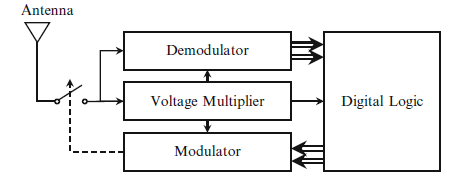
\includegraphics[width=\textwidth]{rfidtagdesign} 
\caption{\label{fig:tagdesign}The design of a RFID tag \cite[p.13]{chipless}} 
\end{figure}

As above mentioned, RFID tags can be categorized in different ways. In contrast to Tamm and Tribowski \ref{classes}, Rezaiesarlak et al. \cite{chipless} describe three different categories \cite[p.9 ff.]{chipless}: Firstly, RFID tags can be distinguished between inductive and radiative (or backscattering-based) tags. Inductive tags are the ones which work below a frequency of 100 MHz and their operating principle is based on inductive coupling between the reader and the tag coil-like antennas. Radiative tags work in the UHF (300 - 3000 MHz) frequency band, providing more reading range as no coupling between reader and dipole-like tag antenna is required. Secondly, there can be differentiated between active and passive tags as mentioned above. Lastly, there are both chipped and chipless tags (see Section Chipless RFID systems \ref{chipless}). 

\subsubsection{RFID readers} \label{reader}

In this section, RFID readers will be explained in detail. 
To start with, one has to imagine existing objects which are tagged with a RFID tag. To implement functionality to these tags and to connect them to a middleware or a backend system, a detector is needed. This detector is the RFID reader which consists of an antenna, a power supply (for passive tags), a microprocessor (to control devices) and an interface for forwarding data to the processing backend system \cite{henrici}. 

Generally, two different types of readers can be distinguished: Stationary and mobile readers. Stationary readers need to be integrated into the existing system architecture by additional middleware \cite[p.133 ff.]{mobile}. Likewise, direct coupling between application systems is not possible because of the amount of data which has to be handled, the lacking ability of being a real-time system and the limited possibilities of RFID readers to produce the required process information. To give an example of the use of stationary readers, they are oftenly used for goods receiving or stock management. Furthermore, stationary readers are fixed to a specific location and need permanent network connection. Additionally, the antenna and reader are spatially separated from each other \cite[p.17 ff.]{fokus}.

On the opposite, mobile readers do not need permanent network connection and are used for instance to query prices in a supermarket. They are usually integrated into mobile devices, connected to laptops, \ac{PC}s or tablets. To connect themselves to an existing system, mobile RFID readers need a device driver which enables the communication between reader and the installed application on the device \cite[p.133 ff.]{mobile}. Furthermore, the antenna as well as the reader itself are integrated into their casing \cite[p.17 ff.]{fokus}.

Nevertheless, there exists the possibility of conntecting various antennas to one reader to extend the range of field.
As mentioned in the section before \ref{tag}, RFID tags and readers communicate via electromagnetism. The reader's detection range depends on the frequency as well as the electromagnetic field \cite{henrici}. In general, four frequency ranges can be differenced: \ac{LF} (125-134 kHz),\ac{HF} (13,56 MHz), UHF (868 MHz-915 MHz) and Microwave (2,54 GHz-5,8 GHz). Each frequency range has its own physical characteristics, such as the needed size of antennas or the read range.

According to Vizinex \cite{vizinex}, an american company with site in Pennsylvania (U.S), HF tags can be used for short read ranges (up to 3 inches). They are usually tagged to tissue samples, blood and critical fluids. Furthermore, HF tags work well in proximidity to liquids as well as human tissues. UHF tags provide longer read ranges and can be detuned by proximity to tissue, fluids and metals. These tags are typically used to track and locate critical medical devices, manage inventories of medical items and track as well as identify patients. Moreover, UHF tags are compatible with worldwide standards and easily deployed because of the compatibility with widely available and competitively priced RFID readers.

Furthermore, each reader has its own electromagnetic field. Such fields are distinguished into near field and far fields: Near fields, also called magnetic or electric fields work with induction and capacitive coupling whereas far fields consist of electromagnetic waves. The measuring unit of electromagnetic fields is called field strength and the maximal field strength depends on national regulations. These national regulations limit the electromagnetic compatibility to avoid disturbing other systems. The functionality of passive tags within near field is different from passive tags in far field. In near field, the tags send data to the reader using load modulation. 

This mechanism does not work in far fields: Here, the sended frequency is backscattered \cite{henrici}.
All in all, readers are able to query tags and to read and write tag data. But the storage of information and the information processing does not take place in readers or tags, but in the middleware or backend systems. These will be explained in the following paragraph.

\begin{figure}
\centering
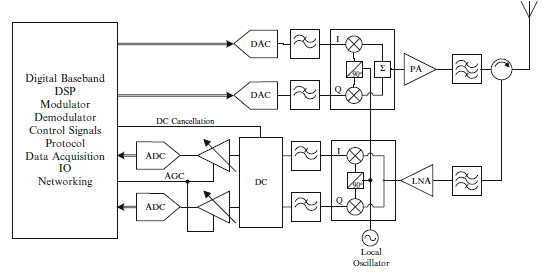
\includegraphics[width=\textwidth]{rfidreaderdesign} 
\caption{\label{fig:readerdesign}The design of a RFID reader \cite[p.17]{chipless}} 
\end{figure}

\subsubsection{RFID backend systems} \label{backend}

As Henrici \cite{henrici} mentions, the backend can be divided into two parts: Middleware and applications. Both of them run on the same computer within the same network which is important for the permanent connection to RFID readers and all existing tags. The advantages of a middleware in this use are that no adaption of appications is needed, an open and neutral interface for other applications is provided. Besides, as the middleware is used to aggregate and filter data, the tags only have to identify objects. As a result, modularity of the system is maintained.

\paragraph{RFID Middleware}

The RFID middleware can be defined as follows: '[...] the software component for preparation and deployment of RFID data which enables the integration of RFID readers and further infrastructure into the operational application systems [...]' \cite[p.20 ff.]{fokus}. According to this definition, there have to be considered three fundamental functions of the middleware: Reassessment, Aggregation and Tranformation. 

To start with, during the reassessment, all received data from the antennas can be redundant or flawed. This redundance is caused by different antennas detecting the same RFID transponder at a time or because one RFID transponder has been detected multiple times during one time frame. Flawed means that transponders were not detected in the intended field or they were detected incorrectly. In second place, aggregation defines the process of summaring all contextual information into one single RFID information ('together into one'). In third place, the term 'transformation' is used by syntactic and semantic means. 

To come to a conclusion, the RFID middleware improves the management of readers by abstracting from technical details. Furthermore, it provides a scalable solution which reduces the unneeded complexity which is transmitted to the users \cite[p.20 ff.]{fokus}.   

\paragraph{Data storage concepts}

Concerning the data management of RFID systems, Tamm and Tribowski suggest three general concepts of storing tag-specific data: 'Data-on-Tag', hybride forms and 'Data-on-Network' \cite[p.22 ff.]{fokus}. 'Data-on-Tag' is a highly recommended method because of the decentral data storage. It improves the user's privacy accessing object-referred information. Moreover, the 'Data-on-Tag' strategy is useful if only relevant and necessary information are contemporarily needed. In addition to that, if the system is not available, the processes can be executed with the tag's information.
Furthermore, 'Data-on-Tag' brings many advantages with it like for instance a raised reliability of the entire system because the processes are decoupled from central system components. 

On the contrary, 'Data-on-Network' implies a central data storage. Further, it can be easily standardized because only the identification number has to be standardized. Further, the only additional requirement remains the working network connection. Mentioning the different data storage concepts in RFID systems brings up another term which is used to detect e.g. product piracy: \ac{CEP}. CEP uses compound read events to detect the multiple capture of one identification number (at different places). If multiple captures of the same identification number are found, the mechanism concludes to a copy of the RFID transponder. 

Actually, data is barely stored on RFID tags because of the limited resources in low-cost tags. It is recommended \cite{henrici} to store tag information on an encapsulated database. As an advantage, databases provide high flexibility to change data or to execute queries without the tags being present. Furthermore, the backend infrastructure should use a \ac{SSL} or \ac{TLS} protocol to ensure a secure transmission of data. Finally, the data would be transmitted and stored in a backend infrastructure on a central storage \cite{henrici}.

\subsection{Functionality of RFID system} \label{chipless}

When developing an RFID system, it is important to think about the unique identification of each object. To enable a reliable identification of objects, only one RFID tag should be attached to each object. The tag itself has a 'read-only' or in some cases 'rewrite' internal memory which enables users to get or change the object's information \cite{ncbi}. 

Secondly, the RFID reader generates magnetic fields to enable the RFID system to locate objects (via tags) within its range. Additionally, the high-frequency electromagnetic energy and the query signal which is generated by the reader triggers tags to reply to the query. Each query can have a frequency of 50 times per second \cite{ncbi}. Thus, it is possible to generate large quantities of data which have to be filtered by supply chain industries. 

Each filter is routed to a backend information system, using a software similar to 'Savant' which is used to control the data. 'Savant' acts like a buffer between the HIS and the RFID reader \cite{ncbi}.
Besides, Tamm and Tribowski \cite[p.18 ff.]{fokus} distinguish between three classifications of RFID systems: 'Close-coupling-systems' ($\le1m$ range), 'Remote-coupling-systems' ($\le1m$ range) and 'Long-range-systems' (>1m range). 

\subsection{Security and Privacy of RFID systems} \label{secprivrfid}

Security and privacy in the healthcare sector is a very important and highly discussed issue. As these are very large issues, which could not be described within a few paragraphs, there will be depicted some examples of threats. In the second section 'Solutions and Methods against Threats' \ref{solution}, five important recommended countermeasures will be described. 
At this point, especially the term of privacy should be defined clearly. According to Tamm and Tribowski \cite[p.90 ff.]{fokus} privacy stands for the right of an individual to keep certain aspects of his life private. Aspects refers to the informational self-determination which should not be controled by further instances, like e.g. systems or third-parties. Additionally, privacy is considered as basic right which is also defined in the Federal Data Protection Act and includes explicitely the protection of personal data.

\subsubsection{Security Problems and Threats} \label{problems}
 
As Henrici \cite{henrici} mentions, there exist two fundamental fears about the RFID technology. The first fear concerns marketing purposes, such as creating very detailed customer profiles which lead to a vast amount of information. Secondly, the technology offers the possibility to keep people under surveillance which implies advantages and disadvantages. As an advantage, the patients' life gets more confortable and companies will be more productive. As a negative result, people's privacy is violated and the application's security is not addressed properly.

Aside from the two fears, Henrici describes several risks of RFID systems, such as the ease of disrupting the service which indicates data security and privacy problems. When talking about security, one should distinguish between security of systems and services and the security of data and information. The last point can only be ensured by secure systems \cite{henrici}. 

In the following, some security and privacy risks using RFID technologies will be explained. To start with, one should think of his passport and the data which is stored on it. The new passports have an internal RFID tag which enables readers nearby the passport to read out all data and to copy them as well. As mentioned in section \ref{tags}, passive RFID tags are cheap, do not have their own power supply and can be read through a nearby reader. So, reading out the passport's data would not be very complex.
Moreover, Henrici mentions product counterfeiting in pharmaceuticals which can cause a lot of harm, like the death of patient's. Nevertheless, the drug market is bound to strong regulations, like for example through the \ac{FDA}. To detect and reduce product counterfeiting, RFID tags need to prove genuineness of original products to patients and should inhibit cloning them.

In his book, Henrici mentions six cases of possible attacks to RFID systems \cite[p.61 ff.]{henrici}. The first attack is called 'Illegitimate reading of data' and describes the possibility of side-channel attacks which use the communication protocol between passive tags and backend systems. As described in section 'RFID backend systems' \ref{backend}, passive tags are used more often and are less expensive than active tags. Nevertheless, the vulnerability of synchronizing each tag with the backend system through a protocol enables attackers to bypass normal protocols so that they can readout all transmitted data.

The second possible attack, Henrici mentions, is called 'eavesdropping of data'. It is caused by the problem of the public and shared communication channel between readers and tags. Compared to 'illegitimate reading of data', everybody near enough the communication channel is able to eavesdrop the conversation because of the use of passive tags. Particularly the 'forward' channel from reader to tag has a stronger magnetic field than the opposite direction which makes it more easily being eavesdropped than the backed one. 

Thirdly, Henrici declares 'cloning or mimicking of tags' as a third threat. His definition of cloning a tag is restricted to creating an exact logical copy of an item which is not distinguishable from the original tag on the protocol level. There might exist some minor differences like the power consumption or time response but the replica cannot be detected with ordinary readers but only with appropriate equipment. The second term 'mimicking' defines the action of infiltrating incorrect data into the RFID system. To show an example, the location might be used for authentication of items. By mimicking a tag, the location can be manipulated and items might appear where they do not exist in reality.

Fourthly, 'recognition of objects' represents another possible threat of RFID systems. In particular, when persons have been detected, they can be used to explore customer habits. Or, in case of patients who wear implants, these might be recognized and the medical information stored on each implant might be abused. In general, each person who carries objects with affixed RFID tags, like wristwatches, shoes etc. might be recognized by an attacker.

Next, the possibility 'tracking of objects' should be considered carefully since tracking of persons can cause many privacy violations. Henrici distinguishes two types of tracking: The first one is called 'direct mapping' and refers to the tracking of RFID wristwatches or glasses. 'Direct mapping' is only possible when the distance between detector and tag is short and the do not exist many tags in one place. Failing that, other items might be tracked by detecting their constellations to each other. These constellations can lead to unwanted creation of movement profiles and the abuse of infrastructure for surveillance by a totalitarian government.

Lastly, Henrici defines the threat of 'causing malfunction' which means that attackers (after having abused one of the above mentioned possibilities) are able to render RFID system malfunctioning. This malfuncionting can be revealed by physical destruction or chemical treatment of tags.  

\subsubsection{Solutions and Methods against Threats} \label{solution}

First of all, data security should always be maintained by the RFID system. But what are the exact countermeasures to prevent an attack on an existing RFID system? When Henrici \cite[p.64 ff.]{henrici} talks about solutions and methods against security threats, he calls them 'Goals of Security and Privacy'. In his book, these goals refer to the possible attacks or threats mentioned in section 'Security Problems and Threats' \ref{problems}. In the following, the countermeasures will be explained. 

'Illegitimate reading of data' can be prevented by controlling data access and ensuring data integrity in RFID systems. False data should be infiltrated because of illegitimate access.
'Eavesdropping of data' can be coped with implementing means for detection and recovering so that the system should keep running even if attackers try to put it out of service. Besides, the integrity of system should always be kept. Another strategy preventing eavesdropping is to maintain data security. Henrici defines a 'good' RFID system to be able to cope with illegitimate reading of data and to treat all the data confidentially.

'Cloning or mimicking of tags' which can be compared to counterfeiting can be prevented by using authenticity mechanisms to identify specific tags. Therefore, RFID tags that can prove their own authenticity should be preferred.

Unwanted 'recognition of objects' can be avoided by developing technical models that provide suitable trade-off of functions. If a function is not wanted by the user, e.g. to allow everyone in the surroundings to read out all RFID attached object, he can adjust this by defining different user roles and rights.

Regarding the realization of the above mentioned goals, there exist many challenges which have to be faced. Henrici \cite[p.66 ff.]{henrici} describes four general challenges which will be explained in the following paragraph. 

First of all, since there are different parties, like e.g. logistic companies and customers which have different needs, the developer has to meet all of their requirements. For instance, the different user needs might be realized by developing different views which depend on the particular user role.

Secondly, developing a secure RFID system is a multidisciplinary challenge \cite{henrici} including six different departments: Computer science (designing communication protocols and the middleware), electrical engineering (realizing the required functionality in hardware and physical layer of communication between tags and readers), mathematics (developing basic cryptographic primitives and theory of probabilities for different areas), economics (adapting the application's constraints imposed by laws of market and assessing real world applicability of approaches), social sciences (including user's requirements, such as privacy and usability) and law (maintaining a legislative basis among people and organizations).

Thirdly, there are more requirements to be faced than 'only' security and privacy, such as low costs or coping with few capabilities and resources. Besides, the enrollment of an RFID system, e.g. in a hospital with many distinctive departments, leads to an inter-organizational operation. To implement this inter-organizational operation, several standards have to be integrated. 

Last but not least, additional requirements have to be considered: Scalability of the system, dependability, low complexity of system, robustness, transparency and usability etc. Henrici claims, that the safeguards should not limit the read range and the speed of reading. Moreover, when using cryptographic primitives, migration paths should be considered.  

\section{NoSQL technology} \label{nosql}

\subsection{Characteristics of NoSQL Databases}

There are many possibilities to store data from application systems. \ac{SQL} can be seen as one of the fundamental database technologies used since the 1980/1990ies \cite[p.137 ff.]{nosql_meier}. The technology of SQL offers advantages, such as consistency, security and integrity of data, as well as the protection of transactions. On the other side, there come along many disadvantages while using SQL. 

To give an example, checking the integrity of data in case of a higher amount of data implicates the need of a higher processing power. Furthermore, facing large-scale development, the efficiency and performance of SQL based systems are decreasing. Moreover, the flexibility and data handling demonstrates another challenge when using SQL. Actually, in practice, the performance is often more important than the consistency, e.g. in social media.    

In the past ten years, there were some NoSQL database technologies coming up. In 2000, these databases were called 'Web-Scale-Databases' because of the need of data storage systems which should handle with the large amount of data of web services \cite[p.221 ff.]{nosql_meier}.

The term NoSQL can be understood as 'Not only SQL' which signifies extension of the existing SQL functionalities. Some data specialists prefer the context of 'no relational databases' which is controversial because of the use of graph databases which deal with relations between nodes.   

In the next section, some examples for the NoSQL data management will be explained and compared to the usual SQL data management. According to Meier and Kaufmann \cite[p.3 ff.]{nosql_meier}, SQL databases are formed on a relation-based model which contains tables with entries. Furthermore, each entry has attributes which are defined by a validating range. A table is defined by its table name, the attribute's name and an identification key. It can have both a column or row order or none of these. The relational model indicates that every table is a set of random tuples and that the relations between data is realized by using tables. The result of SQL queries are always tables which can be uniquely, minimally identified by their identification or primary key.

In contrast to that, the technology of NoSQL offers more possibilities to store data, like for example in key-value stores, column stores, document stores or graph databases \cite[p.16 ff.]{nosql_meier}. These four types of NoSQL databases are also called 'Core-NoSQL-Models'. Besides, other NoSQL database models like object databases, \ac{XML} databases or grid databases are defined as 'Soft NoSQL Models'. 

To give some examples of the 'Core-NoSQL-Models', their fundamental characteristics will be described in the following. The key-value stores (e.g. Cassandra) provide the simplest way to store data by using an identification key and a list of values. Document stores (like e.g. MongoDB \ref{mongodb}) store the data in form of structured text data like \ac{JSON} or XML. In contrast to key-value stores, document stores have a pre-defined structure but are schema-free which means that the data structure can be changed over the time. 

Graph databases (e.g. Neo4J) introduce a new way to store data: It introduces a graph-based model. Each graph consists of nodes and edges which connect the edges and demonstrate their relations. Each node can have concepts and object. Both, nodes and edges have a label and can contain properties. Each property contains an attribute and a value. The query language for graph databases is called 'Cypher' \cite[p.16 ff.]{nosql_meier} which is a declarative language. Users of Neo4J and other graph databases are able to specify their retrieval query by defining nodes and edges. By evaluating all possible paths (or connections between nodes and edges), the database system calculates all requested patterns.   

Generally, NoSQL technologies are popular for their high availability as well as their protection against system failures by using different replication concepts, e.g. 'Consistent Hashing' \cite[p.11 ff.]{nosql_meier}. In addition, NoSQL is characterized by its vertical and horizontal aligned scalability, its weak or non-existent restrictions concerning schemas and data models. Along, NoSQL databases offers simple data replication and easy access through API \cite[p.221 ff.]{nosql_meier}.  

Edward and Sabharwal discuss the pro and cons of NoSQL technologies in their book \cite[p.17 ff.]{mongodb_edward} which will be given in the next paragraph.
On the one hand, NoSQL offers high scalability, manageability and administration (such as automated repairs, distributed data etc.), low cost and flexible data models. But on the other hand, using NoSQL factors like maturity, limited query capabilities, administration (installing and maintaining solutions) and limited expertise (developer and administrator community are limited).

A \ac{DBMS} defines a software which describes, stores, queries data independently from an application \cite[p.2 ff.]{nosql_meier}. It consists both of a storing and managing component. The storing component is composed of all data which has to be stored in organizational form and their description. The managing component contains a querying or manipulating language to evaluate data and to change them, such as access control units and an user interface. When it comes to the use of web applications and a heterogeneous data pool in real-time, SQL databases are often not suitable for these problems. In this case, a NoSQL database should be considered. 

\subsection{Excursus: BIG DATA} \label{bigdata}

The term 'Big Data' has been emerged during the past 10 years. Due to the enormous data pool, e.g. in social networks or user analysis, which is not easy to manage with usual software tools, new data technologies were needed. As a solution, NoSQL technologies have been arised. Furthermore, Big Data refers to unstructured data which comes from different sources \cite{nosql_meier}. 

Edward and Sabharwal define Big Data as the following: It is a '[...] term used to describe data that has massive volume, comes in a variety of structures and is generated at high velocity. This kind of data poses challenges to the tradtitional \ac{RDBMS} used for storing and processing data. Big Data is paving way for newer approaches of processing and storing data.[...]' \cite[p.1 ff.]{mongodb_edward}. Furthermore, Edward and Sabharwal refer to an explosion of data created by smartphones, social networking sites, in short words from various sources in various formats, such as video, text, speech, log files and images. The type of stored data varies by its 'sector', e.g. retail and whole sale, administrative parts of government, financial services mainly generate text or numerical data (including customer data and transaction information). 

On the other hand, in the healthcare, manufacturing, media and communication sector especially multimedia as well as image data is produced. To give an example, X-Rays, CT and other scans dominate the storage volumes in healthcare. 

Another important point, when it comes to large amounts of data is the consumation model or the various sources from which data is produced and subsequently consumed \cite[p.6 ff.]{mongodb_edward}. Edward and Sabharwal declare two models: In the old model, few companies produced data and all others (users, clients, etc.) consumed them. But nowadays, they claim that '[...] all of us produce data and all of us consume them [...]' \cite[p.6 ff.]{mongodb_edward}. This creates a new challenge of developing multiple user data models and make the existing data management system more scalable than in the past. 

\subsubsection{Velocity, Variety, Volume}

When talking about Big Data, often there come up three descriptive terms: Velocity, Variety and Volume.

Velocity refers to the real-time high-speed evaluation of the upcoming data \cite{nosql_meier},  also known as 'real-time insight' \cite{mongodb_edward}. Edward and Sabharwal describe velocity as 'Data in motion' \cite[p.7 ff.]{mongodb_edward}. Besides, they mention that if data cannot be processed at required speed, it losses its significance. For many companies and organizations, it is very important to process data both when it is moving as well as when it is static. 

Variety means that there are distinct formats of data: structured (e.g. integer, string), semi-structured and unstructured data \cite{nosql_meier}. Edward and Sabharwal describe variety as 'Data in many forms' \cite[p.7 ff.]{mongodb_edward}. As mentioned in the last paragraph, data can vary from simple text files, log files, streaming videos, photos, meter readings, stock ticker data, PDFs and many other unstructured format.   

The last characteristic of Big Data, volume, deals with the high amount of data \cite{nosql_meier}. Edward and Sabharwal describe volume as 'Data in many forms' \cite[p.7 ff.]{mongodb_edward}. They see a reason for the higher volume in businesses becoming more transaction-oriented and the number of transactions is increasing. Moreover, more devices are connected to the internet which increases the size of data.

Calolas et al. refer to challenges like e.g. dealing with tremendious amounts of data, unstructured data (diversity of \ac{OSN}) as well as the complexity to challenge analyzing social networks data \cites{trends_nosql}.

\subsubsection{Usage of Big Data}

Edward and Sabharwal depict five large use cases of Big Data which will be explained in the following \cite[p.9 ff.]{mongodb_edward}. Firstly, visibility of data is very important for many companies. For example if data is accessible across departments of a company, it can be readily integrated. This reduces the search and processing time, improves product quality according to present needs \cite[p.9 ff.]{mongodb_edward}. 

Secondly, discover and analysis information is another use case for large amounts of data. After capturing detailed data, e.g. of inventories, employees or customers, new information or patterns will be discovered and analyzed. The captured information and knowledge can be used to improve processes and performance of companies \cite[p.9 ff.]{mongodb_edward}. 

Thirdly, segmentation and customizations can be effected by means of using Big Data. To give an example, the segmentation of customers is based on various parameters and can aid in targeted marketing campaigns or tailoring of products to suit the needs of customers \cite[p.9 ff.]{mongodb_edward}. Fourthly, Big Data can aid, improve or automize decision making by using Big Data analytics which can minimize risks and uncover valuable insights. Lastly, Big Data can strengthen innovations in existing products by using data gathered for actual products \cite[p.9 ff.]{mongodb_edward}.    

\subsubsection{Big Data challenges}

The issue 'Big Data' not only offers many possibilities or use cases, but also faces many challenges \cite[p.11 ff.]{mongodb_edward} which will be discussed in the consecutive paragraph. To start with, Edward and Sabharwal indicate policies and procedures which can constrain the use of Big Data. They refer to data privacy, security, intellectual property of organizations. Furthermore, in order to comply with various statutory and legal requirements, Big Data has to face the challenge of data handling, which includes issues around ownership and liabilities around data. In second place, the access to data has to be controlled precisely.

Since some data might be available to third parties, the gaining access poses a legal, contractual challenge. After that, in order to handle Big Data, new tools as well as technologies have to be built specifically. Moreover, there might exist legacy systems in several organizations or companies which have to deal with Big Data. Besides, there exists a lack of experienced resources in these newer technologies which is also a challenge to.

Most of the legacy systems are designed to work with structured data \cite[p.11 ff.]{mongodb_edward}. Since legacy systems are created to perform fast queries and analysis on tables and columns, they cannot be used to hold or process Big Data (which contains unstructured data). Another important point is the data storage for Big Data. Currently, in many companies, data is stored on big servers (using \ac{NAS} or \ac{SAN} systems) \cite[p.11 ff.]{mongodb_edward}. With the increasing data, the server size and backend storage size has to be increased. 

Lastly, when handling with Big Data, data processing is very important . Usual algorithms in legacy systems are designed to work with structured data and are limited by data size. Therefore, legacy systems are not capable of handling processing of unstructured data, high volumes of data, speed etc. To capture value from Big Data, the deployment of newer technologies are needed. 

\subsubsection{Big Data technologies}

Edward and Sabharwal propose several ways of implementing Big Data technologies \cite[p.12 ff.]{mongodb_edward} which will be depicted in this paragraph. To begin with, Big Data needs new storage and processing technologies which are designed for large, unstructured data. After that, other technologies like parallel processing, clustering are emerging in order to handle Big Data. Additionally, large grid environments, high connectivity and high throughput offer new fields for software developer and data scientists. Finally, cloud computing and scale-out architectures have been arised during the last years.

\subsection{Example for using NoSQL Databases: 'Socii System'} \label{socii}

To give an example of the use of NoSQL technologies, the next section will focus on explaining a developed system 'Socii'. 'Socii' was developed from Jroge Daniel Calolas, Alda Lopes Gancarski and Pedro Rangel Henriques. In their article 'Online Social Network Analysis Visualization Using Socii' \cite[p.218-228]{trends_nosql}, they describe the several technological challenges they faced during development but also the benefit of this social network analysis and its scientific importance. In short words, 'Socii' is a system which enables the analysis and visualisation of social networks by helping \ac{OSN} users to exploit and understand their own networks through a user friendly interface. During development, Calolas et al. were facing four main principles: simplicity, accessibility, OSN integration and contextual analysis.

One big problem before developing of 'Socii', Calolas et al. mention was the observation of social structures and the analysis of these networks. By establishing 'Socii', the authors Calolas et al. wanted to proprose to fill the gap or struggle that OSN users have in understanding their network. To give an example of these struggles, there were three main topics, Calolas et al. were facing: 'how relationships evolve along the time', 'what role play these friendships within the network' and 'how they can analyze and visualize their networks based on social properties (such as mutual relationships, geographical positions, personal tastes and preferences or hobbies)' \cite{trends_nosql}. 

\subsubsection{Structure and flow of data analysis and visualization systems}

When introducing 'Socii' as an social analysis tool, Calolas et al. also talk about several tasks and steps during the process of data analysis and visualization systems. Firstly, data has to be extracted (through APIs, web crawlers and web scrapper. Secondly, data is achieved which requires careful selection of relevant data to store \cite{trends_nosql}. In order to have an efficient system that provides good structure for data analysis, one needs to select the data carefully. In the third step, data is explored by defining of what one user wants to do with the data. Furthermore, during this step, there are two important questions: What are the applications that can be seen for the stored data? How can the system digest and transform data in order to make it useful and interesting for the end user? 

Lastly, in the fourth step, data is visualized which means the kind of presentating or showing the transformed data is chosen by the user. Particularly, the work of the data scientist has a huge impact on the end user. In generals, the data visualization targets a general audience.  
By extension, 'Socii' affirms web availability, OSN's  integration, contextual analysis and being a trade-off for such gains the system performance.

\subsubsection{Main functionalities of 'Socii'}

One of the main functionalities of 'Socii' is information extraction and data mining \cite[p.223]{trends_nosql}. These include extracting some user networks form given OSNs by calling web crawler modules which then return the extracted information. After that, an extraction manager sends the extracted data through a simple data mining process in order to data normalized before it is stored in the database (MongoDB). Web crawlers are implemented in Python and the crawling operations are performed using XPath selectors to extract the information that are needed to build the network.

Generally, the main functionalities of 'Socii' amount to OSN contextual netowrk analysis (with relatively low complexity) \cite[p.227]{trends_nosql}. Moreover, 'Socii' intends to integrate data from different OSNs by processing a set of node properties displayed together with the network structure. Roughly, Calolas et al. implemented three features of 'Socii'. To start with, 'configurable, parameterized analysis' enables users to select several metrics upon a given network. 

Consequently, 'clear, intuitive social graph visualization and interaction' refers to the visual web component of 'Socii' which provides users a set of visual features (coloring, node discovery etc.). Thirdly, 'Socii' offers an 'organized overview upon SNAs and OSN data' which include visual components that aggregate SNAs metrics and OSNs information. Thus, users are able to cross information from both and can derive conclusions from intersecting the information \cite{trends_nosql}. 

\subsubsection{Limitations of 'Socii'}

As shown in the last paragraph, 'Socii' offers many features to analyse Big Data especially in social networks. Nevertheless, Calolas et al. depict some limitations and disadvantages which will be explained in the following. 
There exists a technical and architectural struggle of feeding the system through an extraction pipeline built on top of the web crawlers. This is known and proved by a very slow, limited and error-prone method for data extraction and the authors call it the 'bottleneck' of their built system \cite [p.227]{trends_nosql}. 

\subsubsection{Future outlook of 'Socii'}

According to Calolas et al., 'Socii's implementation should be completed to work with other OSN's. Furthermore, it can be extended to perform evaluation and validation of system with users having accounts in several OSNs and several profiles. 


\chapter{Development of RFID application for management and tracking assets and drugs}
\label{Kap3}

The third and last chapter of this Bachelor Thesis gives information about the development process of the RFID tracking application. In the following, the system's requirements \ref{requirements} will be described as well as the first drafts will be given \ref{firstconcept}. Additionally, all used platforms and technologies are mentioned in section \ref{platforms}. Then, the specific development process \ref{app_development} is depicted which demonstrates the software's architecture introducing some diagrams. Lastly, several planned tests as well as their test results are discussed in section \ref{tests}.

\section{Proposed solution of application}\label{requirements}

\subsection{Aim of developed application}

The aim of the proposed system is to improve logistics and the management of drugs in hospitals. Considering the risk of errors or mistakes that might occur when administering drugs to patients, the developed mobile application can prevent these situations. Furthermore, when patients are in a critical situation, the system offers the possibility to respond faster to emergencies as well as to improve patients' monitoring. Finally, the placement and usage of medical assets can be pursued and controlled better. 

The above mentioned reasons lead to the necessity of disposable, low cost sensors which might be tagged to patients, drugs and medical assets. Moreover, there has to be established a network between the mobile devices as well as the reader and the synchronizing software. 

\subsection{Scope of developed application}

\begin{figure}
\centering
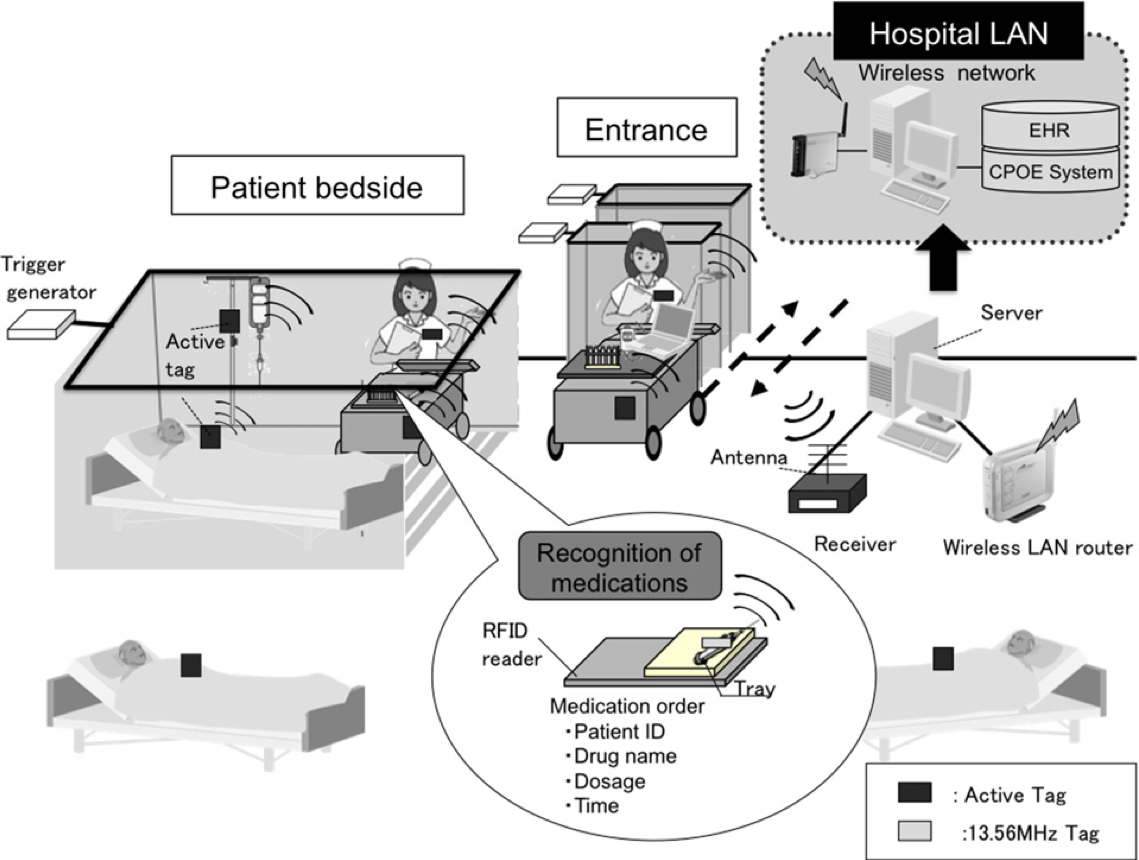
\includegraphics[width=\textwidth]{existing_apps} 
\caption{\label{fig:existing_apps} Existing RFID systems, based on 13.56 MHz short-range, inductive RFID tags} 
\end{figure}

In the past, the existing RFID systems for management and logistics in hospitals were mostly based on 13.56 MHz short-range, inductive RFID tags.
Figure \ref{fig:existing_apps} gives an example of an existing RFID solution for management in hospitals. This caused several advantages as well as disadvantages. On the one hand, as an advantage, using 13.56 MHz short-range, inductive RFID tags is a mature technology which is reliable. Further, the past solutions imply low-cost RFID tags which are easy to use. 
On the other hand, the disadvantages of the mentioned solutions are their complex infrastructure and the short-range. 

Therefore, the present bachelor thesis introduces the use of 868 MHz frequency band while using a similar RFID architecture as the ones already tested and deployed. As an advantage of using 868 MHz frequency band, the proposed solution implies a longer range, wider coverage and the required hardware can be simplified. Further, the proposed solution of this bachelor thesis provides a mobile application for users which can be run on tablets and smartphones. 

In a nutshell, this bachelor thesis modifies the \ac{RF} hardware as well as the front end whereas the back-end and core network remains the same.

\subsection{First concept of application} \label{firstconcept}

Figure \ref{fig:first_draft} describes the very first draft of the workflow of the application. Actually, it is not very precise but should help to describe the general scope of the medication tracking system. 
At the top of the picture, there is an Excel program which stores all data of the database and converts them into *.CSV files. These converted files should be imported into the running MongoDB instance on the PC. 

On the same computer is running Matlab which is connected with the RFID reader. All along, MongoDB and Matlab are synchronizing each other. Beneath the PC, the figure shows the RFID reader which is connected to four antennas. At the bottom of figure \ref{fig:first_draft}, there are drawn four zoned antennas. Each zone can be seen as a different area or room and can represent a different state, e.g. 'entering' or 'leaving' the stockroom. In the bottom left corner, there can be depicted RFID tags which pass one antenna after another. Each time, an antenna recognizes a tag, it sends the transmitted information to the reader which transfers the data to Matlab.  

\begin{figure}
\centering
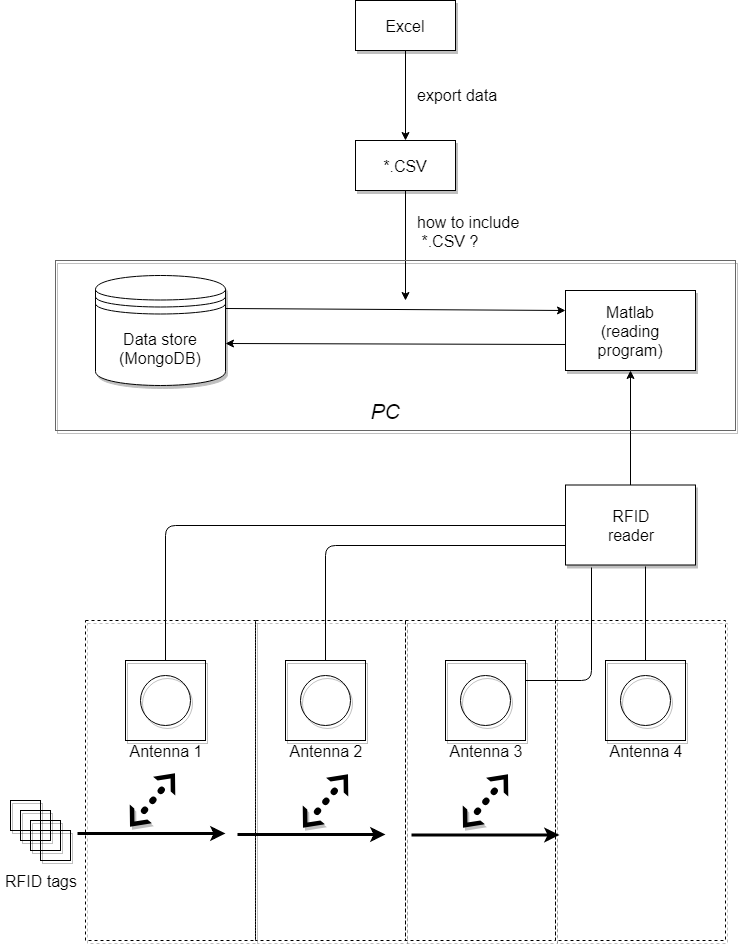
\includegraphics[width=\textwidth]{first_draft} 
\caption{\label{fig:first_draft}The first draft of the developed system} 
\end{figure}

This first concept was changed due to the 'MongoDB' plugin, which offers Matlab \cite{matlab_mongodb}. This is much easier than exporting all received data from Matlab in *.CSV format and then including it into MongoDB as *.CSV data. Furthermore, it supports developing a very fast and real-time application which enables a higher data integrity because of the direct connection to the database (see also figure \ref{fig:app_architecture}.  

%talking about platforms in general, to get a common understanding 
\section{Used platforms and technologies} \label{platforms}

This chapter focusses on explaining the used technologies and frameworks for developping the mobile RFID application. In the following, the framework 'Nativescript' which can be used for native mobile development will be explained. After that, a further section will discuss the technology of NoSQL and will compare it to SQL database technology. This section will also depict MongoDB, a document store. Finally, the Impinj RFID reader will be presented. In the last section \pageref{app_development} of this chapter the challenges as well as the user scenarios will be shown. 

\subsection{Native Development with NativeScript} 

There exist several ways to create a mobile application. But the challenge is to develop a consistent solution for the existing systems, like e.g. Android or iOS.
To face the challenge of developing a hybride solution which can be run both on Android and iOS devices, Nativescript has been established as an open-source project from Telerik in the last years \cite{nativescript}. 

The free and open source technology enables developers to easily build cross-platform native apps with either Javascript, Nativescript or by using Angular \cite{nativescript}. 
Regarding its design philosophy, Nativescript was designed to be approachable to developers from various backgrounds \cite{nativescript}. Moreover, it was designed to be both performant and giving access to native APIs, such as Android or iOS.

Figure \ref{fig:nsarchitecture} gives an impression of the general architecture of Nativescript applications. When developing such applications, one of the given frameworks can be used (e.g. '\{N\} Core', Angular or Vue). Additionally, several Nativescript plugins can be selected. Below the 'NativeScript Core Modules', there are located the 'NativeScript Runtimes' which have direct access to the Native system. By running several commands on the NativeScript \ac{CLI}, the developed Nativescript application can be executed on any physically connected device as well as on the installed emulator or in the cloud. 

\begin{figure}
\centering
\includegraphics[width=\textwidth]{ns-architecture} 
\caption{\label{fig:nsarchitecture}The architecture of NativeScript Applications, adopted from \cite{nsarchitecture}} 
\end{figure}

NativeScript applications can also be developed, built and run on the 'NativeScript Playground' \cite{nsplayground} which enables independent development. Moreover, NativeScript Playground is easier to handle because the development machine does not have to be prepared. Generally, by offering a user-friendly surface, NativSscript Playground is appropriate for beginners who start developing native mobile application.

\paragraph{NativeScript Application Logic}

\begin{figure}
\centering
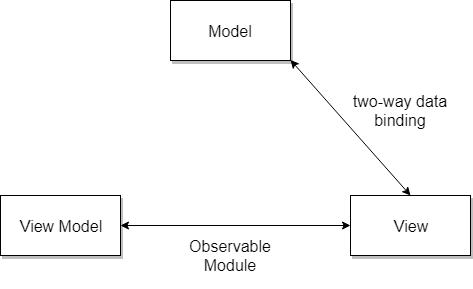
\includegraphics[width=\textwidth]{mvvm_ns} 
\caption{\label{fig:mvvm}The MVVM application logic, adopted from \cite{nativescript}} 
\end{figure}

Nativescript has a \ac{MVVM} application logic (see figure \ref{fig:mvvm}). In contrast to the popular \ac{MVC} application model, Nativescript offers two-way data binding by using the 'Viewmodel' \cite{nativescript}. In every NativeScript application, the model defines and represents data. After that, the data are bound to the view which represents them in a XML file. The 'ViewModel' contains the application logic and exposes all data to the view. 

Between Model and View, data can either be bound as one-way (default setting, the target property updates when a change in the source property occurs) or two-way data binding (all changes in the directions target-source and source-target will be transmitted). To enable the two-way data binding (see figure \ref{fig:mvvm}), the NativeScript Observable Module has to be implemented. 

In the NativeScript Documentation \cite{nativescript} declares the model files as 'Code Behind' because they have the same name as the view file and are written in Javascript or Typescript. By adding attributes to any XML element in the view file, methods can be implemented in the related model file (in Javascript). 

\subsubsection{NativeScript Sidekick}\label{Native}

Nativescript Sidekick is a solution to run the developed application on unsupported platforms in the cloud. It uses both the local build infrastructure and the cloud build service. Nativescript Sidekick offers users to develop with the provided starter templates, to use verified plugins and to build the app in the cloud. Furthermore, Nativescript Sidekick enables developers to debug, test and refactor their application. 
To search for plugins and to manage these, developers can use the Nativescript Marketplace \cite{nsmarket}.

\subsection{NoSQL Technology: MongoDB}\label{mongodb}

As mentioned in section Document Store \pageref{documentstore}, this type of NoSQL database provides high availability, scalability and partitioning options \cite[p.25 ff.]{mongodb_edward}. Nevertheless, there are some disavantages when using MongoDB or any other document stores: For instance, both consistency and transactions are not supported. 

In contrast to relational databases, MongoDB does not consist of tables and rows, but of collections containing documents which make it both flexible and scalable \cite[p.25 ff.]{mongodb_edward}. Collections can be compared to tables in SQL but are schemaless. Instead of having one unique schema within the same collection, every document can have its own set of fields, and common fields can store different values across documents.  

All data is stored in \ac{BSON} documents which assures that related data is placed all together in one place. BSON documents are JSON documents in binary-encoded format. It is the extended form of the JSON data model and is fast, high traversible and lightweight \cite[p.31 ff.]{mongodb_edward}. Moreover, JSON/BSON documents contain schema-less models. Each documents stores data as key-value pairs, where the value can be left blank (see above, disadvantage of consistency). Thus, users of MongoDB have to ensure and check the consistency of their data when adding new data.

One characteristic of MongoDB is the {\_} ID (key) which can be compared to the label or name of a colum in RDBMS. If not explicitely specified by the user, a unique value is automatically generated and assigned  to it by MongoDB. Basically, the key value is immutable and can be of any data type except arrays \cite[p.31 ff.]{mongodb_edward}.

Queries in a MongoDB database use the keys ({\_} ID) in documents which makes it possible to query documents spread across multiple servers. 
MongoDB uses primary-secondary replication, where the primary replication accepts the write requests. To be more precisely, if the write performance needs to be improved, the mechanism of sharding can be used. 

Sharding means that data will be split across multiple machines which are enabled to update different parts of datasets \cite[p.25 ff.]{mongodb_edward}. Besides, this mechanism is automatic in MongoDB, so that as more machines are added, the data is distributed automatically.

\subsubsection{Limitations and possibilities of MongoDB}

There are many advantages and disadvantages, limitatiions and possibilities when using MongoDB. The following paragraph will discuss these and give some examples.

Generally, MongoDB offers many features which MySQL does not. To give an example, MongoDB supports secondary indexes, atomic updates at a per document level. Additionally, queries can be executed by using query documents. Furthermore, MongoDB provides replica sets which are based on master-slave replication with automated failover. After that, MongoDB provides a built-in horizontal scaling. Finally, MongoDB can be run everywhere (e.g. on Cloud, \ac{VM}, servers etc.) because it is written in C++. 

Another feature of MongoDB are 'Capped Collections' which store documents in the inserted order. When the capped collection reaches its storage limit, documents will be deleted from the collection in the inserted order (analogous to \ac{FIFO} principle). Capped collections are often used for log files in order to get these automatically truncated after a certain size. In the end, capped collections guarantee preservation order data in the insertion order \cite[p.31 ff.]{mongodb_edward}.

On the other hand, in contrast to relational databases like MySQL, MongoDB does neither support JOINs nor fully generalized transactions \cite[p.25 ff.]{mongodb_edward}. Secondly, when using MMAPv1 as storage engine, the used space is too large because its data directory files are larger than the database's actual data \cite[p.226 ff.]{mongodb_edward}. For that reason, it is recommended to use MongoDB's WiredTiger storage engine which compresses all files and reduces the storage size by 50\%. Moreover, once a collection is dropped diskspace is automatically reclaimed (unlike MMAPv1 engine).

Thirdly, when using MongoDB BSON documents, their usage is limited the size, nested depth and field limits of the specific document \cite[p.228 ff.]{mongodb_edward}. After that, namespaces as well as indexes are limited, for instance the maximum size of indexed items has to be1024 bytes. The number of indexes per collection must not exceed 64 indexes. Moreover, the usage of sharding is limited \cite[p.230 ff.]{mongodb_edward}. Therefore, if shards were implemented too late, a slowdown of servers is caused because splitting and migration of chunks takes time and resources. Thus, Edward and Sabharwal  recommend to shard a collection before reaching 256 \ac{GB}. 

Next, when using MongoDB, there exist some security limitations because the database does not provide authentication by default. This enables every user which is connected to the database server, to read, change, add and delete data. In addition to that, the connections to and from MongoDB are not encrypted by default. Therefore, when starting the database server on a public network, it is recommended to use encrypted communications. Therefore, Edward and Sabharwal propose the SSL-supported build of MongoDB (which is available as 64-bit version) \cite[p.230 ff.]{mongodb_edward}. 

What is more, using MongoDB implicates write and read limitations, such as case-sensitive queries and type-sensitive fields since there is no enforced schema \cite[p.231 ff.]{mongodb_edward}. For instance, users have to ensure the correctly used type when adding new data. By the same, replica sets which can be used to ensure data redundancy, are limited by the number of the members in every set. When using such replica set, one member acts as a primary member whereas the rest acts like secondary members (a node needs the majority of votes to become primary).

All in all, MongoDB provides many possibilities but also limitations. Generally, it should be clarified that MongoDB is neither adequate to be used in a highly transactional system nor in business intelligence applications where issue-specific databases shall generate highly optimized queries. Finally, it should not be used in applications requiring complex SQL queries. Instead, it is recommended to store high amounts of data and to ensure its availability at any time. 

\subsubsection{MongoDB: Best Practices}

Edward and Sabharwal suggest some 'best practices' when using MongoDB \cite[p.234 ff.]{mongodb_edward} which will be explained briefly in this paragraph. 
First of all, the correct hardware should be chosen. For example, the more internal memory is given, the better the performance of the MongoDB application. Another important point is the CPU: for its productivity, MongoDB needs a fast \ac{CPU} clock speed, as well as a high \ac{RAM}. Moreover, using SATA SSD and \ac{PCI} ensures good price as well as performance results.

Concerning the best practices in coding, Edward and Sabharwal propose to set a correct data model. Further, they recommend avoiding application patterns that lead to unbounded growth of document size as well as to design documents for future which are better to handle with MongoDB's drawback. Besides, documents should be created with an anticipated size where ever applicable. But the most important point when coding is to check data consistency \cite[p.234 ff.]{mongodb_edward}. 

With respect to the data safety and how to provide it in the deployed MongoDB database, Edward and Sabharwal both replication and journaling of data \cite[p.234 ff.]{mongodb_edward}. Furthermore, the repair should be the last resort for recovering data in case of a server crash. Basically, they recommend to always specify a timeout with assuming the command and to run the MongoDB server instance in trusted environment with access control.

Likewise, concerning the administration of MongoDB, Edward and Sabharwal submit to perform instant-in-time backups of durable servers and to use repair in order to compact databases \cite[p.234 ff.]{mongodb_edward}. Correspondingly, managing the replication log is of administrative concern \cite[p.240 ff.]{mongodb_edward}. 

Respecting sharding, it is important to select a good shard key. Moreover, Edward and Sabharwal recommend using three config servers in production deployments to provide redundancy \cite[p.240 ff.]{mongodb_edward}. 

Finally, Edward and Sabharwal introduce 'monitoring' which means that every MongoDB system should be proactively monitored to detect unusual behaviours \cite[p.240 ff.]{mongodb_edward}. To put this into practice, MongoDB's free hosted monitoring service, MongoDB Cloud Manager (which contains a dashboard view of the entire cluster metrics, can be used. Besides, MongoDB itself provides 'mongostat' and 'mongotop' to gain insight into the performance of the database instance (e.g. operation counters, active working sets etc. are shown). 

\subsection{Impinj RFID Lector and Antenna}

The developed system was tested and run on a Speedway R420 RAIN RFID READER \cite{speedway} with four antenna ports (extendable to 32 antennas with an Impinj Antenna Hub \cite{speedway}) and a flexible read range (short and long-range reads are supported). According to the manufacturer's web page \cite{speedway}, the Speedway R420 RAIN RFID READER can be connected to Impinj Autopilot technology which automatically optimizes the reader's operation for its environment. Furthermore, there can be downloaded the appropriate software from the Impinj web page \cite{speedway}.
In the following section, there will be given some information about Impinj, RAIN RFID as well as some example use cases. 

\subsubsection{General Information}

To start with, RAIN RFID will be presented. RAIN RFID is a global alliance promoting universoal adoption of UHF RFID technology \cite{rainrfid}. It can be compared to NFC Forum, WiFi Alliance or Bluetooth SIG. Moreover, RAIN RFID uses a GS1 UHF Gen2 Protocol which is ISO-standardized (18000-63). According to the alliance, the term RAIN shall represent the node between UHF RFID and the cloud where RFID-based data can be stored, managed and shared. Several RAIN RFID uses reader to read and write a tagged item, manage data and take action.

Impinj (also known as NASDAQ:PI) enables wireless connection of multiple everyday items, such as apparel, medical supplies, automobile parts, luggage etc. The Impinj platform uses RAIN RFID to deliver timely information about all items to the digital world (application systems) \cite{impinj}.

\subsubsection{Examples}

Impinj mentions some example use cases when implementing the Speedway R420 RAIN RFID READER: Inventory Management, Asset Tracking and enhanced shopper experience. 
The DeRoyal Industries, Inc. which was founded 1973 is a medical device facturer\cite{deroyal}. With the aim of improving clinical quality and economic health of customers, DeRoyal provides surgical devices, unitized delivery systems, orthopedic supports and bracing wound care dressings.

One of their software solutions is the system 'DeRoyal Continuum Safe' \cite{deroyal}. By using the Impinj platform and RAIN RFID, DeRoyal Continuum Safe automatically captures and tracks data from medical supplies in the operating room, emergency department and catherterization lab. The solution includes packaging which is tagged with RAIN RFID tags. According to DeRoyal, the system provides many advantages, such as reducing the time staff spend managing supplies so that they can focus more on patient care. 

Besides, DeRoyal Continuum Safe improves billing accuracy for supplies used during procedures. After that, the likelihood of infections is reduced by ensuring the availability of necessary supplies. Lastly, DeRoyal achieved to provide a data-driven supply chain management \cite{deroyal}. 

\subsection{Matlab}

According to Dr. Knuth's 'Art of Computer Programming', Matlab is an interpreted language, usually used without an compilation step \cite[lesson 1]{introduction_matlab}. Actually, the Matlab code is converted into machine code by an interpreter as the program is executed. Together with Java, Matlab counts to the high-level languages which on the one hand enables a faster code development but on the other hand limits the speed of execution. Matlab provides a large number of functions for common complicated operations in scientific computing (including engineering and analysis) and technical calculation.

Matlab provides important terminology, like e.g. variables (which contain three fundamental types: characters, real numbers, complex numbers), arguments, commands, command line, scripts, functions as well as comment \cite[lesson 1]{introduction_matlab}. 
One of the most common features of Matlab is its 'Debugger' \cite[lesson 8]{introduction_matlab} which is very usefull for detecting unobvious errors.

Simulink is an add-on product to Matlab which enables an interactive, graphical environment for modeling, simulating, analyzing of dynamic systems \cite[p.313 ff.]{simulink}. Further, it enables rapid constructions of virtual prototypes to explore design concepts at any level of detail with minimal effort \cite[p.313 ff.]{simulink}. For modeling, Simulink provides a GUI for building models as block diagrams so that users are able to produce a 'up-and-running' model. Finally, Simulink is integrated with Matlab and data can be easily shared between the programs.

\subsubsection{Mathworks}

Mathworks is the leader of software development of mathematic calculation, especially for engineers and scientists \cite{mathworks}. Found in 1984, Mathworks is employing more than 3500 employees in 15 countries. Mathworks' headquarters is Natick, Massachusetts, U.S. All Mathworks products are used in various sectors, e.g. automation, airspace, communication, electronics, industrial automization etc. Its main purposes are modeling and simulation which are realized through Matlab and Simulink.

\section{Application development} \label{app_development}

\subsection{Progress of development}

The development process can be devided into four large steps which will be described in the following section. 

To begin with, during the very first weeks one work package was learning how to create a NativeScript application from scratch. This phase included making experience with the common NativeScript templates, views and framework logic as well as the data binding and data handling.

As a second work package, the challenge of how to connect the NativeScript application to the backend (MongoDB) was faced. As a first solution, the connection to the MongoDB server was implemented using HTTP request/response. But in practice, this solution offered the problem that only one client could access the database. But in reality, there might be at least two devices (used by a nurse or doctor) which have to be connected to the database. For that reason, a socket connection (using the Socket.IO library) was established. With this technology, it was possible to connect multiple clients to the server instance and to synchronize all data in real-time.

After that, the third work package introduced the handling of Matlab, its connection to MongoDB and to the Impinj RFID reader. In order to connect to the RFID reader, the Impinj Octane SDK was implemented. By using the Impinj Octane SDK, it was possible to configure several functions for each antenna of the reader. This enables a precise identification of each antenna as well as the precise location of each detected item or drug. To give an example, antenna 1 could be set as hallway or floor whereas antenna 2 stands for patient's room. 
Concerning the connection between RFID reader and MongoDB, there exists a MongoDB plugin for Matlab. This provides several methods to connect to a MongoDB server and to retrieve and change the data from a specific database. Concluding these two implemented functionalities, Matlab serves both as a detection and information medium.

The last large work package refers to the challenge of establishing a stable connection between all components (RFID reader, MongoDB database, NativeScript application and mobile devices). Therefore, two networks had to be created. The first network (LAN) connects the development laptop (MacOS) where both the NativeScript application and MongoDB database are running to the Windows PC where Matlab is running. Due to the use of .NET libraries in Impinj Octane SDK, Matlab had to be installed on a Windows PC. Another solution would be to run Windows on a VM on the MacOS developer machine, but unfortunately the RAM as well as disk space restricted the functionality of the VM. The second network that was installed was a private WLAN which connected all mobile devices (smartphones and tablets) with the MacOS developer machine. This connection enables receiving and transfering all data from the MongoDB database into the mobile app. To be precisely, the WLAN provides a secure connection to all mobile devices by using a \ac{WPA2}.

\subsubsection{Challenges during development} \label{challenge}

During the development, many difficulties and challenges had been faced. The following section will focuss on some big problems during development.
To start with, the setup of the development environment of a NativeScript application was complicate because for example on Windows computers there cannot be installed XCode. So, the only solution to develop and run the application both on Android and iOS devices was to use a MacOS computer or to execute the application on Nativescript Sidekick (using its cloud build service). Furthermore, during the setup of Android Studio and the runtime environment of Android on MacOS caused other complications. To give an example, sometimes having installed the Android \ac{SDK} 25 the Android \ac{AVD} Manager required exactly the same version being installed on its virtual device. 

Another challenge was the real-time synchronization of the mobile application with MongoDB server was difficult. Firstly, a HTTP request/response was implemented to connect the mobile device with the RFID reader and the database. But using the HTTP request/response was a very static and non-scalable solution (only one device was enabled to connect to the server). Furthermore, refreshing the page was not automated. Thus, another solution had to be considered. Finally, a Socket.IO connection was implemented between both server and client. Socket.IO enables automatic two-way data synchronization and cannot be compared to HTTP Request/Response. By opening a Socket connection between the server and all clients, it was possible to run the application on various mobile devices without any complication. 
After that, another complication was the connection between MongoDB, Matlab and the NativeScript application. This was solved by using a server instance which both connects the database as well as the Nativescript application. Section \ref{section_architecture} explains the exact implementation and the used architecture to connect all system components. 

\subsubsection{User Scenario}

Figure \ref{fig:appfunctionality} gives an example of one user scenario. The figure shows two treatment rooms in a hospital, both equipped with a RFID antenna. In the hallway, there are two additional antennas applied which are connected to the RFID reader. When passing one room, the nurse or doctor will roll a trolley with the needed drugs (all marked with a RFID tag). If the trolley is near to the RFID antenna \#4, it will send the current drug information to the RFID reader which synchronizes them with the computer and the tablet or smartphone. When entering a treatment room, RFID antenna \#3 or \#2 receive the tag's information and synchronize them similarly as before.

At the bottom of the figure, there is a drawn a intranet/internet connection. This means, that the system can be both set up in the local intranet (which enables a higher privacy and security) as well as in the internet. In the end, each RFID antenna can signify a different action, e.g. antenna \#4 = 'medication will be administered', antenna \#3 and \#2 = 'medication is dosed to patient X', \#1 = 'medication has been dosed successfully'.

\begin{figure}
\centering
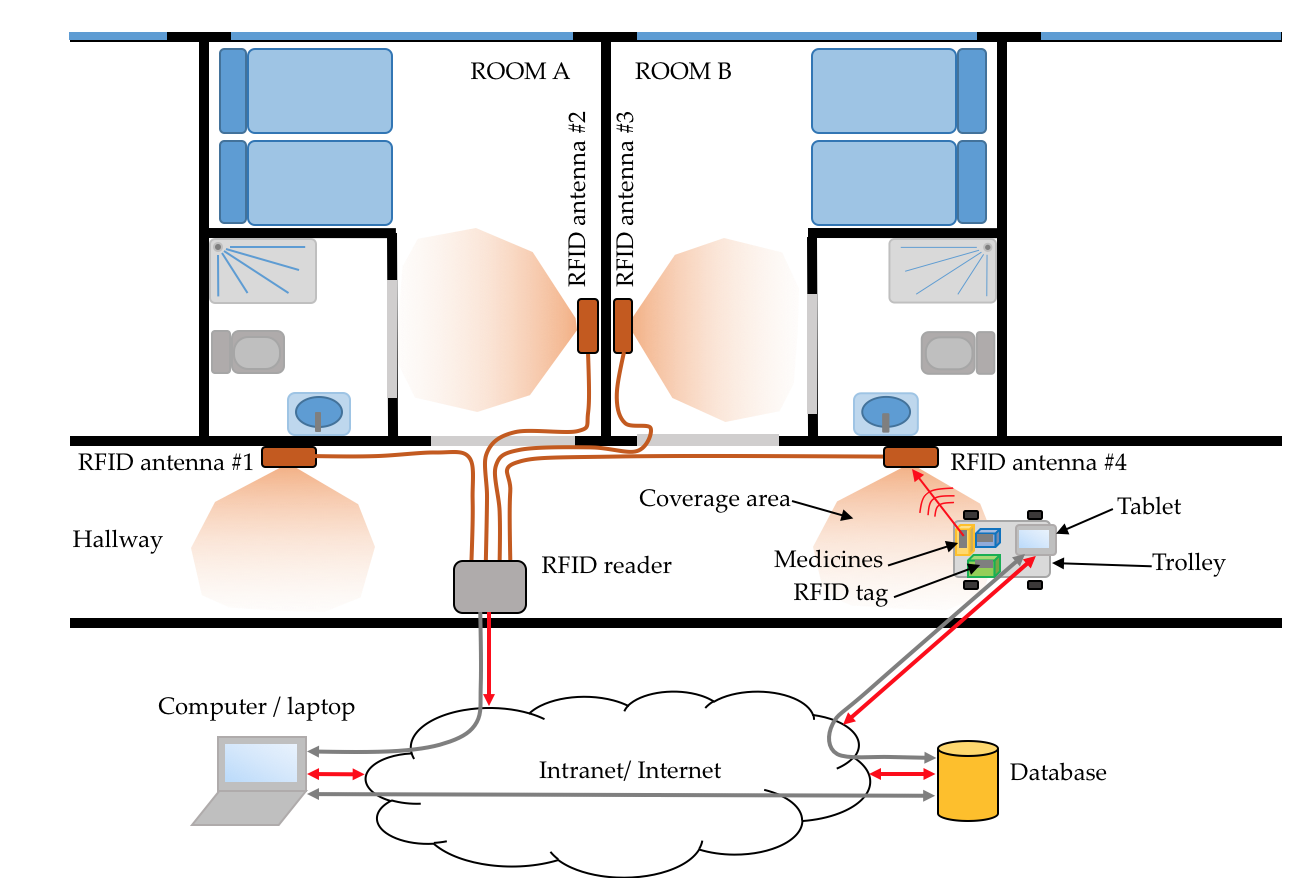
\includegraphics[width=\textwidth]{app_scenario} 
\caption{\label{fig:appfunctionality}User scenario of RFID application} 
\end{figure}

Figure \ref{fig:app_screenshot} shows three screenshots of the developed application. The left picture shows the start screens containing a list of all drugs which were detected by the RFID reader and are stored in the database. The screenshot in the middle shows the screen after selecting one drug of the start page. It gives further information of the selected item. Each drug is stored with an 'ID' (which is the same as the RFID tag number). The 'Countrycode' attribute refers to the country-specific number of each drug. For example, in Germany 'Aspirin' has a specific unique code which is called \ac{PZN}, and contains a 7- or 8-place number (e.g. 04114918). The 'Location' attribute describes the exact location of a drug and refers to the location system in the stock (e.g. in pharmacies). The information 'Timestamp' refers to the last time a drug was detected. The value on the right side of 'Timestamp' is the default value for storing timestamps in MongoDB. If another date format is required, this can be easily defined in the MongoDB schema definition. The last information about the selected drug, named 'Event', represents the information about a drug being detected by one of the antennas or administered to a patient. If the nurse or doctor selects the button 'Administer to patient', the system checks, if the selected drug is permitted to be administered to the patient in the room or not. If it is permitted, the information about the administrated drug will be stored in the database and the content of the 'Event' changes to 'Administered to patient in room XX'.

\begin{figure}
\centering
\subfigure[Start page of application]{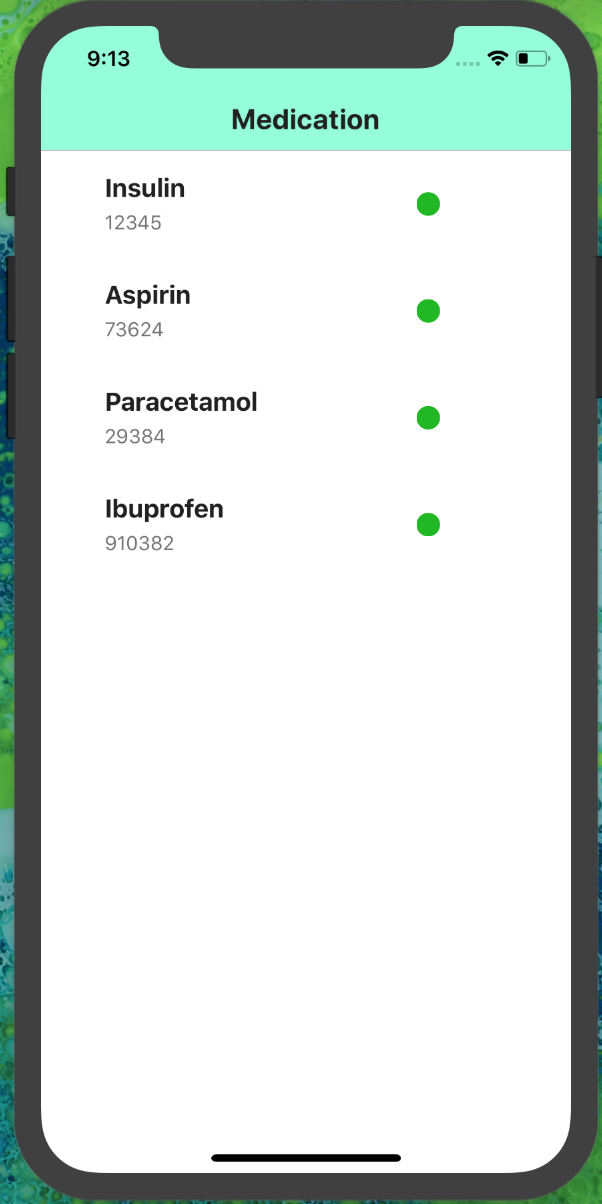
\includegraphics[width=4cm, height=8cm]{Mainview}}
\subfigure[Item information page]{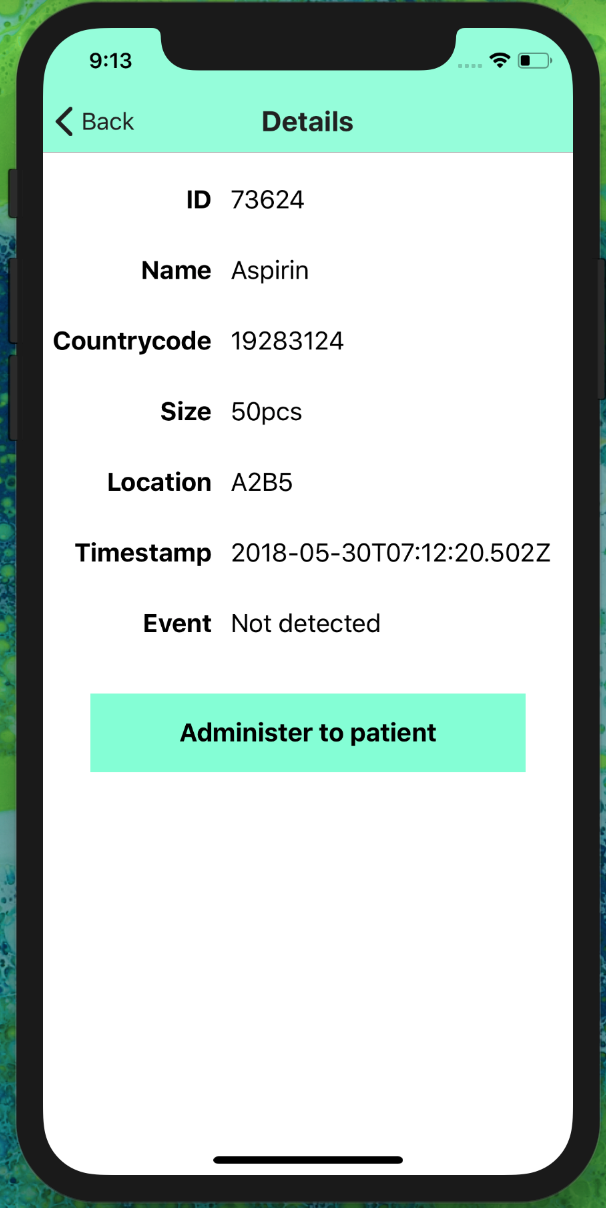
\includegraphics[width=4cm, height=8cm]{Detailview}}
\subfigure[Information about administered drug to patient]{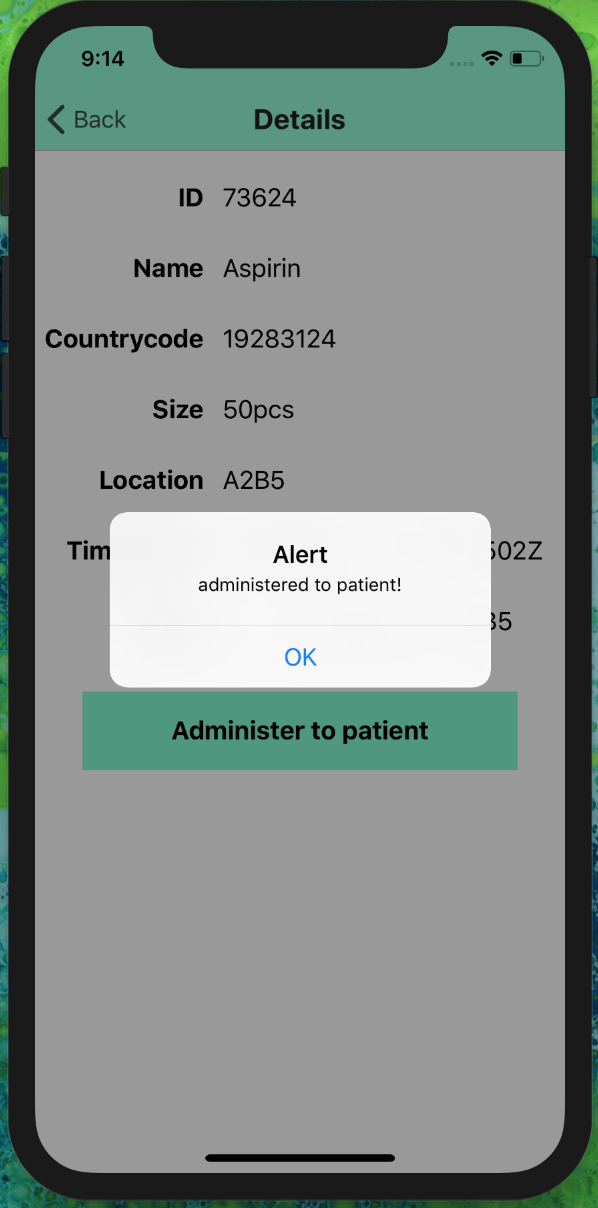
\includegraphics[width=4cm, height=8cm]{administeredView}}
\caption{\label{fig:app_screenshot}Layout of application, Screenshot of iOS Simulator}
\end{figure}

\subsection{Software Architecture} \label{section_architecture}

The following section focusses on the system's architecture which can be seen on figure \ref{fig:apparchitecture}. In the top right corner, there are displayed drugs and patients which can be tagged with a RFID tag. When approximating an antenna of an RFID reader, information about medication (e.g. stock availability ect.) are transmitted. At the same time, the RFID reader registers the detected tag and captures its information using Matlab. Matlab synchronizes the transmitted information with the MongoDB database. When receiving new drug information, the server instance sends the data through a Socket.IO connection to the client (smartphone or tablet). Synchronously, all data is transmitted and displayed on the mobile device.

\begin{figure}
\centering
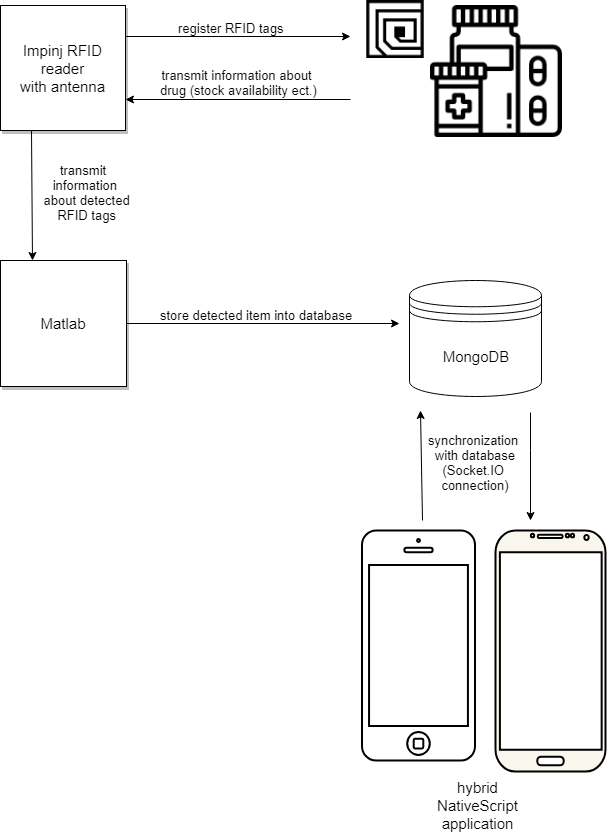
\includegraphics[width=\textwidth]{app_architecture} 
\caption{\label{fig:apparchitecture}The developed system architecture of the mobile RFID application} 
\end{figure}

\subsubsection{Datamodel}

Concerning a useful datamodel, the following figure \ref{fig:datamodel} reflects the outline of the developed MongoDB document related to its context and the MongoDB database. As described in figure \ref{fig:app_screenshot}, 'Details', each drug entry contains information about its ID, name, countrycode, size, location, timestamp and event. All documents are pooled in a drugs collection which forms a part of medication database. This data model can be extended for example by other collections containing information about several equipment or patients. 

\begin{figure}
\centering
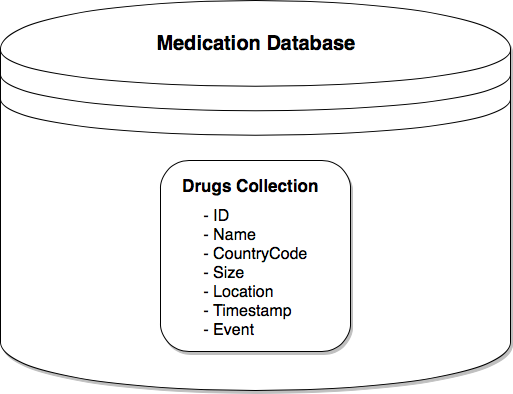
\includegraphics[width=8cm, height=6cm]{Mongo_DataModel} 
\caption{\label{fig:datamodel}Applied data model} 
\end{figure}

\subsubsection{\ac{LAN} Architecture}

Figure \ref{fig:hub_architecture} represents the realization of connecting all relevant components into one LAN. There exist two networks: On the one hand, the LAN between RFID reader, laptop and desktop PC. On the other hand, a local network between the laptop and various mobile devices, like smartphones or tablets is established. The only connecting point between both networks is the laptop with the IP 169.254.1.2.

At the top of figure \ref{fig:hub_architecture}, there is a '5-Port-Ethernet-Hub' which enables connecting up to five different devices or computers via ethernet. 
On the left of the picture, there can be depicted the RFID reader which has the default IP of 169.254.1.1. Each time, when detecting a RFID tag, the RFID reader sends the information to Matlab which is running on the desktop PC with the IP 169.254.1.3. 

After receiving the detected RFID tag's information, the desktop PC transmits the data to MongoDB database running on the laptop with the IP 169.254.1.2. 
The purpose of the second local network between laptop and mobile devices is to execute the NativeScript app and to visualize currently detected RFID tags in the app.

\begin{figure}
\centering
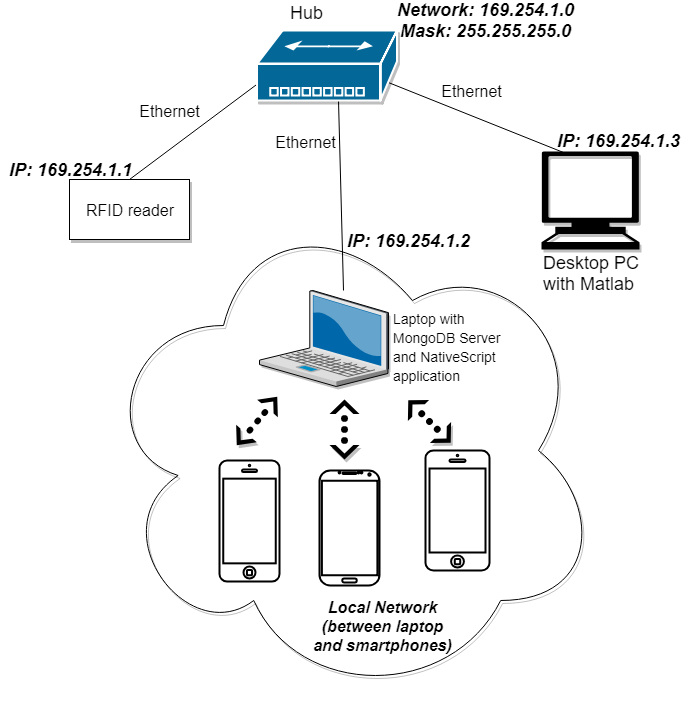
\includegraphics[width=\textwidth]{hub_architecture} 
\caption{\label{fig:hub_architecture}The LAN architecture of the developed system} 
\end{figure}

\subsubsection{Reading Process in Matlab}

The following section focusses on the reading process which is implemented in Matlab. Matlab uses the Impinj Octane SDK \cite{octanesdk} which easily connects the RFID reader to Matlab. The usual reading process in Matlab can be seen in figure \ref{fig:reading_matlab}. In the top left corner of figure \ref{fig:reading_matlab}, after starting the Matlab code, a setup method triggers the initialize method. 

After initializing, Matlab starts reading tags during a predefined time (t). In a loop, every time is read. When reaching the limit of time, the method eventhandlerChanged() is executed. EventhandlerChanged() notices the changes in the detected tags and triggers a new action 'store data'. After that, analogous to the first concept of the system (see section \ref{firstconcept}), the *.mat data is converted into *.csv data and as such exported. In the most current version of the system, the two last actions (conversion and export) are brought together and data is directely transfered into the MongoDB database. 

\begin{figure}
\centering
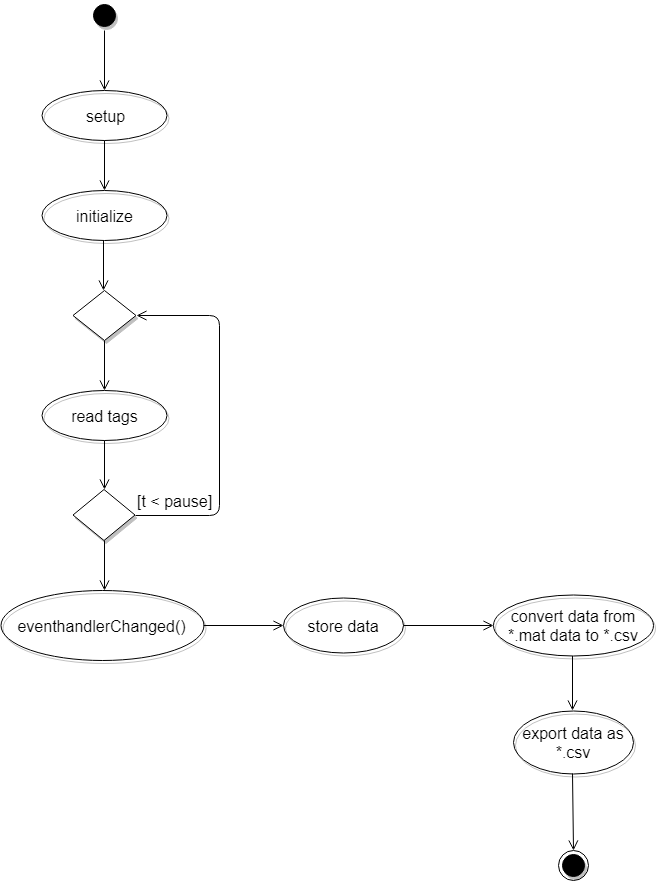
\includegraphics[width=\textwidth]{reading_matlab} 
\caption{\label{fig:reading_matlab}Activity diagram: reading process in Matlab} 
\end{figure}

\section{Tests of system}\label{tests}

\ac{HUCA} which is situated in Oviedo, was created in 13 December 1989 and depends on the 'Servicio de Salud del Principado de Asturias' \cite{huca}. Since 28 February 1990, HUCA has the character of an University Hospital due to the cooperation with the university of Oviedo as well as 'Insalud' and Principado de Asturias, established in 'la Orden'. 
HUCA provides 944 beds, 25 operating suites, 238 rooms for external surgical as well as two gamma cameras (\ac{SPECT}/\ac{TC}) \cite{huca}. Altogether, HUCA is divided into 43 medical subjects, such as Alergology, clinical analysis, clinical biochemistry, surgery, Nephrology, Neurology, Rehabilitation, prevention of work-related risks, radiodiagnostics etc. 

Besides, HUCA forms a part of the 'unit of national reference for work-related illnesses of the respiratory system'. Together with the 'Hospital Monte Naranco', 'hospital del Área Sanitaria IV' and with reference to \ac{SESPA} 'Servicio de Salud del Principado de Asturias' and finally the 'Instituto Nacional de Silicosis', HUCA promotes research on the subject of respiratory disease and its preventions measures.

Figure \ref{fig:permission} shows the permission letter, signed by the director Gloria Herías Correal of HUCA on 8 May 2018 in Oviedo.
The tests are planned for June 2018, an exact date is not fixed already (effective 18 May 2018). 

\begin{figure}
\centering
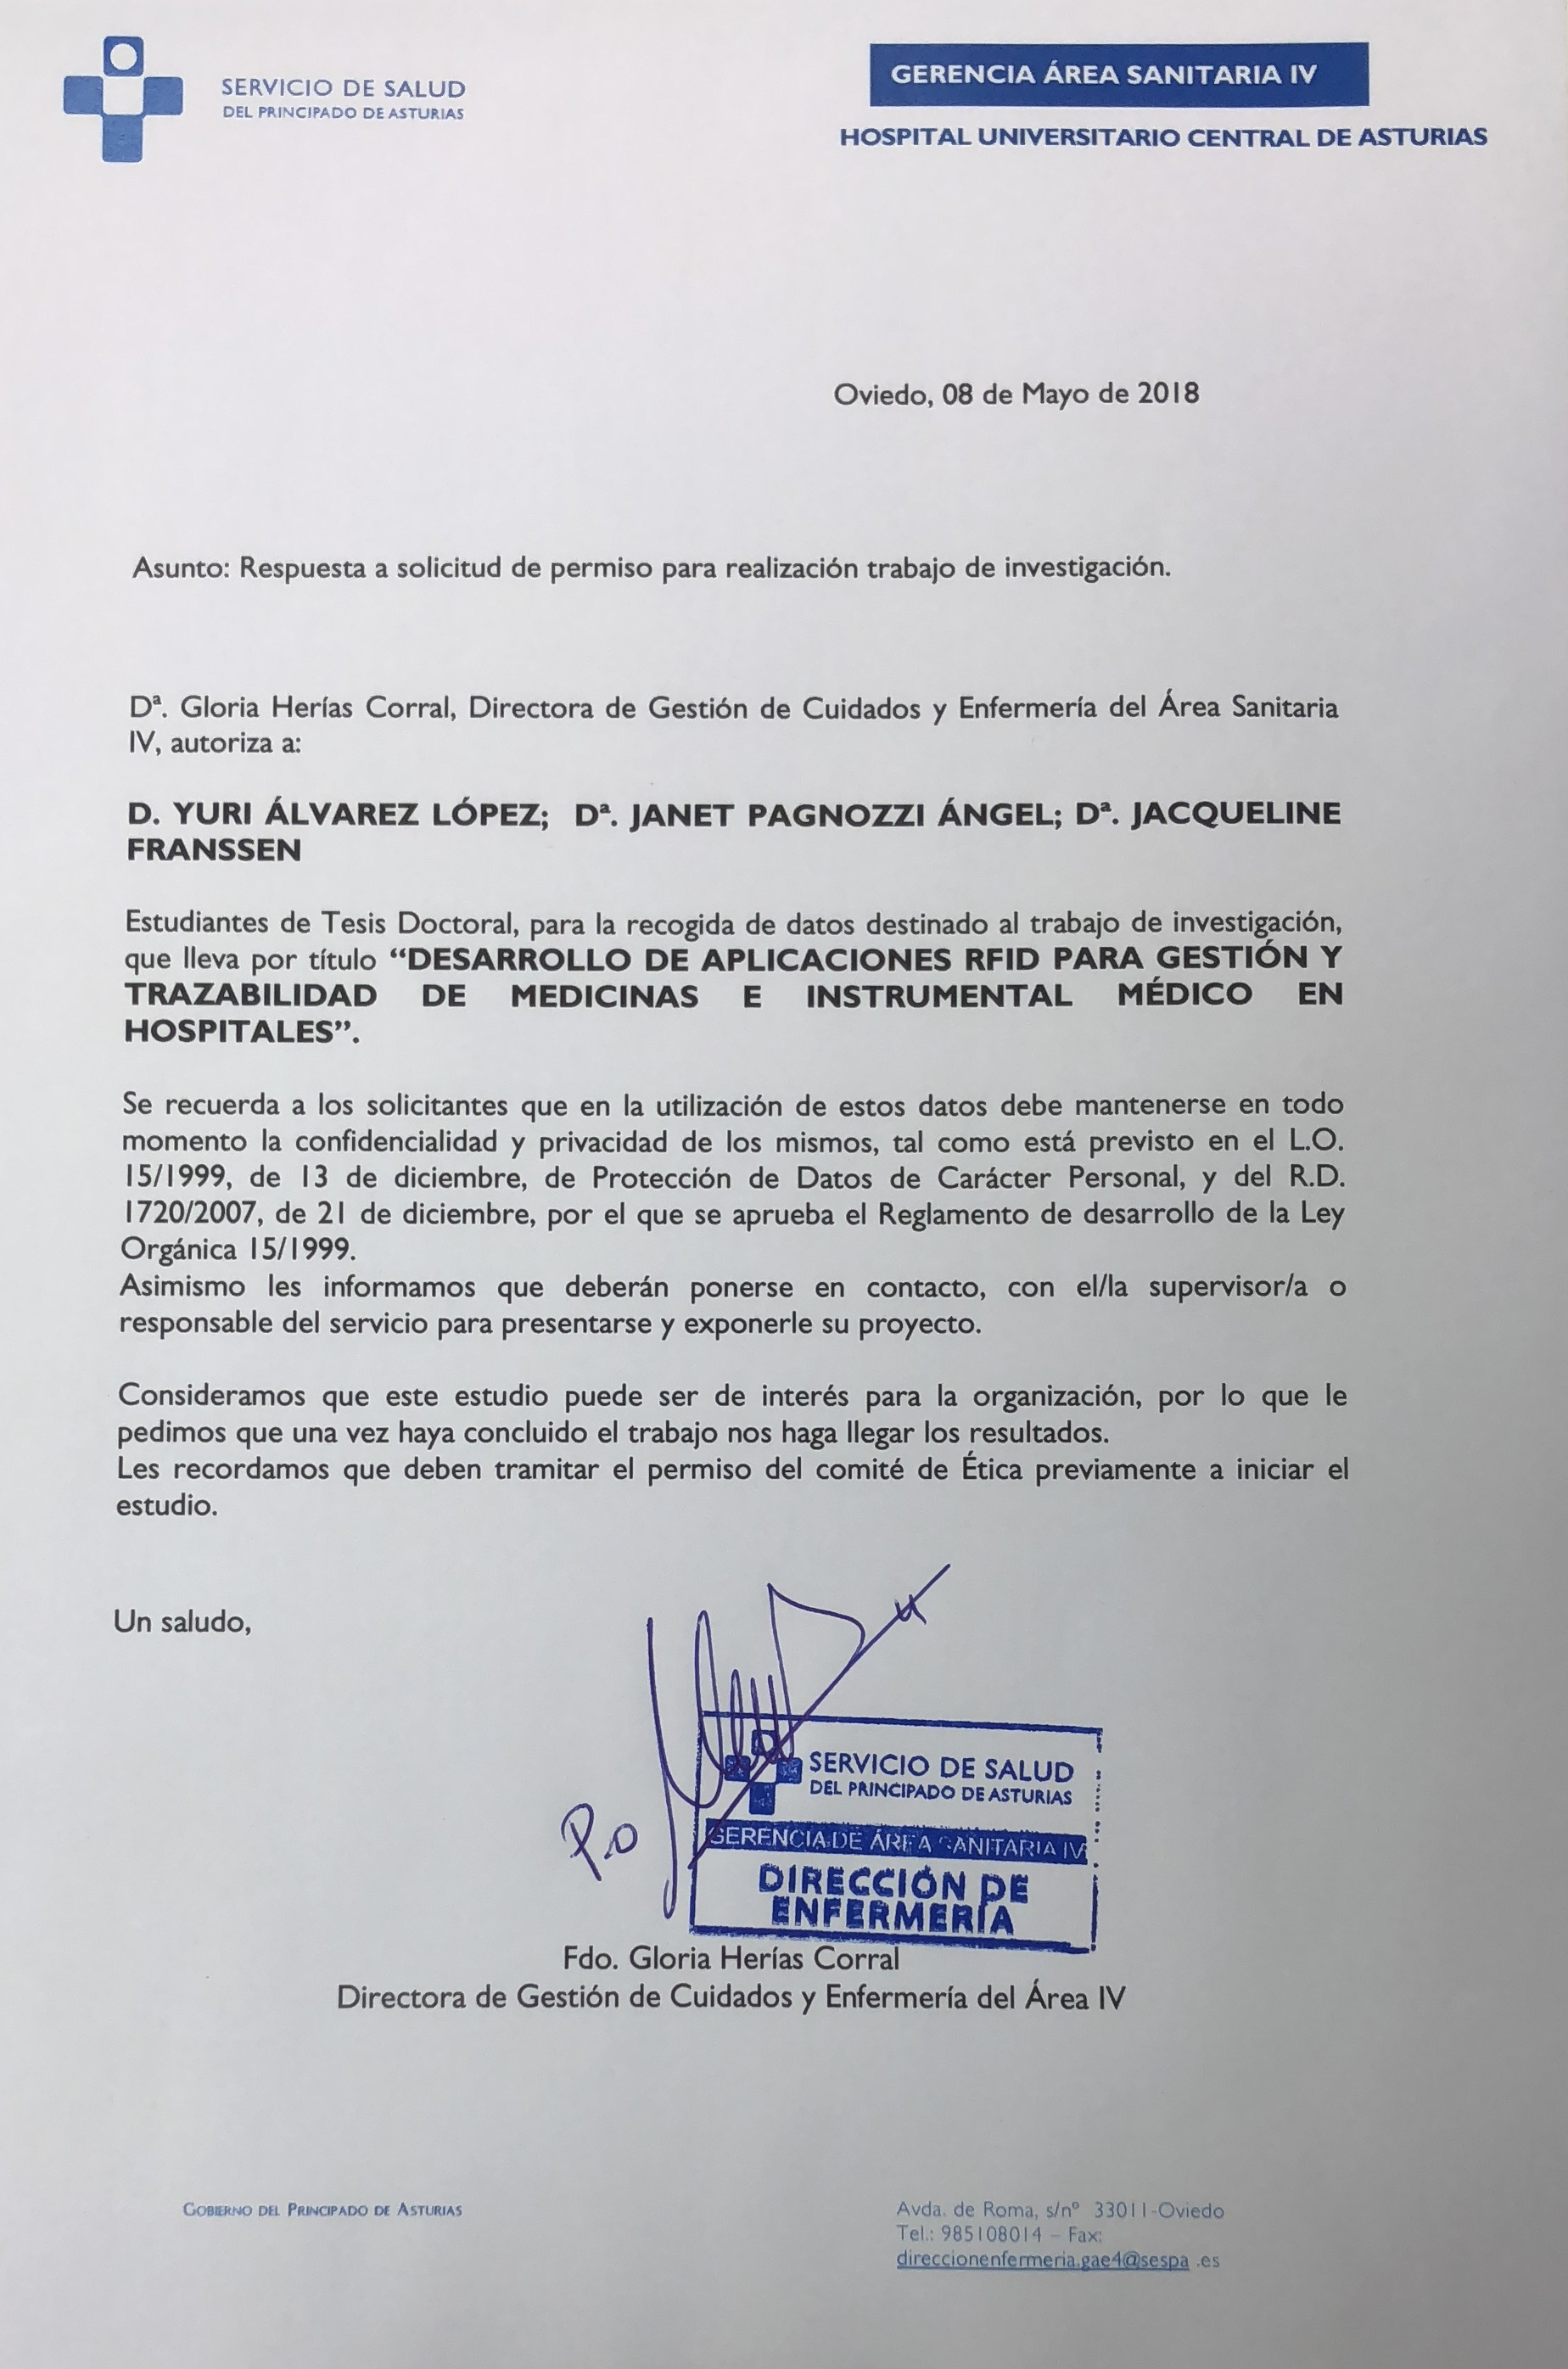
\includegraphics[width=\textwidth]{permission_HUCA} 
\caption{\label{fig:permission}Permission letter about application tests in HUCA} 
\end{figure}

\subsection{Planned tests of system}

\subsubsection{Test scenario}

The following section describes a test scenario which is planned to be administered in HUCA. 
To begin with, one has to imagine, that a nurse has to administer several drugs to many patients in a hospital. In the past, there where many cases, where nurses dismissed or administered medication to patients incorrectly. To prevent those errors and to improve patient's safety, the nurse can control and capture each time she is administering a drug to a patient. The system will check if the selected drug (which was detected in the patient's room) is valid and if it can be administered to the patient. For example, the nurse is walking with a transport trolley (containing several drugs) on the hallway of a certain department in the hospital. On the hallway, there are two antennas which are connected to a reader which is installed nearby. When passing these antennas, the detected drugs will be automatically stored into the MongoDB database and displayed on the mobile phone or tablet. 
When entering the patient's room, a second antenna detects the drugs and transmits the signal to the reader which receives the information about the location of the drug ('drug X detected in room 314'). After that, if the nurse wants to administer a drug, the system checks whether it was already administered and whether it is permissible. After having administered the selected drug, the event will change to 'already administered in room X' and will be stored in the database. 

\subsubsection{Functional tests}

In order to test the real-time synchonization, all entries in the database were deleted and the application was refreshed (by using the pull-to-refresh plugin). After five seconds, the alert dialog which explains that there are no entries in the database and no detected drugs is displayed (tested 06 June 2018).

\subsubsection{Device test}

The application was tested on four devices including both tablets and smartphones. During development, mainly the iOS simulator was used to rapidly execute and synchronize the application. Since installing a prototype app on an iOS device requires several developer certificates and some configuration steps, it was easier to use the included simulator which is offered by XCode. 
Later, when the app could be executed without throwing any errors, it was installed and tested on an iPhone 7 (256 GB and iOS 11.4, 15F79). Furthermore, it was installed on an iPad (iOS 11.4) and ran successfully. 
Moreover, the app was tested on two Android devices: a Samsung Galaxy S3 (Model: GT-9300, Android Version 4.3, smartphone) as well as a Samsung GT-P5110 (Android Version 4.2.2, screen size: 10.1'', tablet).

the following figure will be replaced by beautiful screenshots from android app

\begin{figure}
\centering
\subfigure{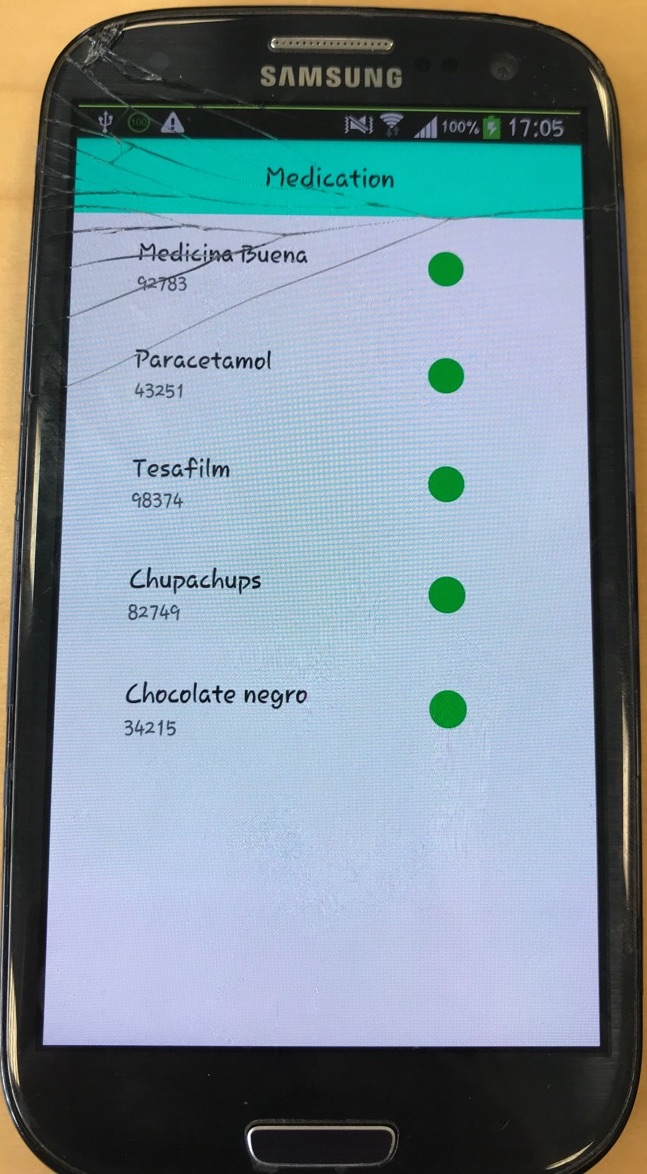
\includegraphics[width=4cm, height=8cm]{s3_01}}
\subfigure{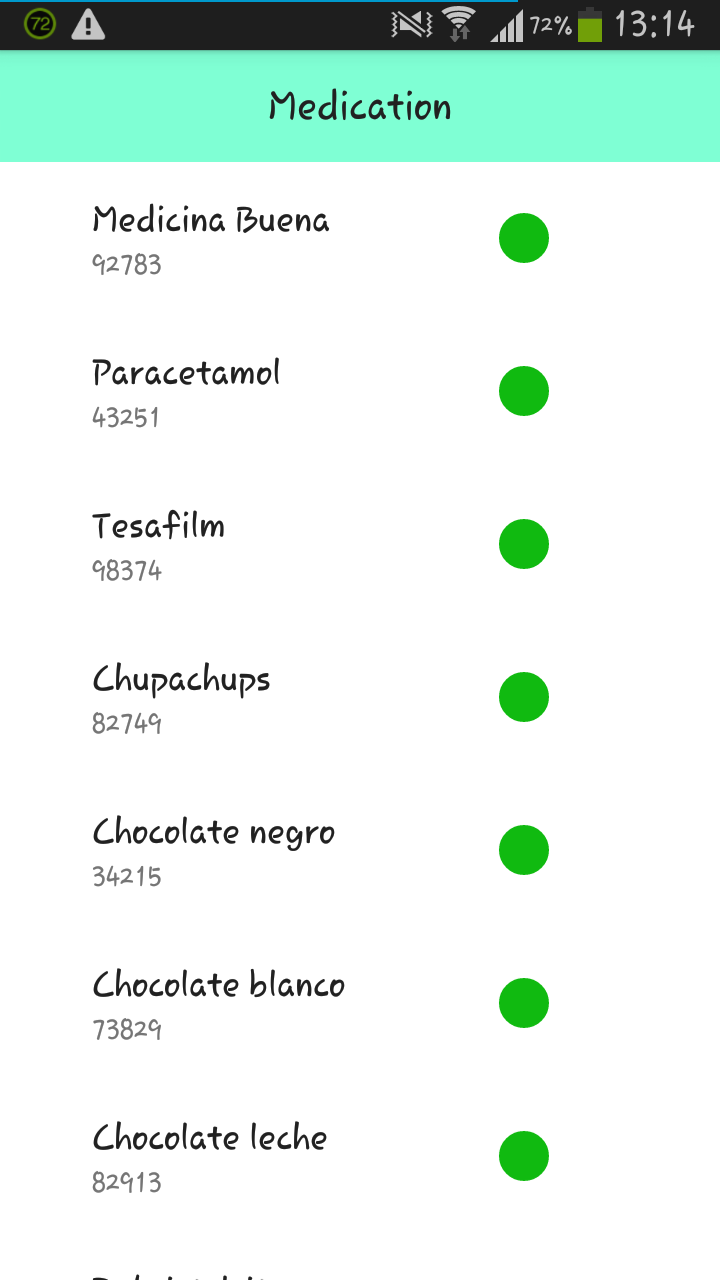
\includegraphics[width=4cm, height=8cm]{s3_02}}
\subfigure{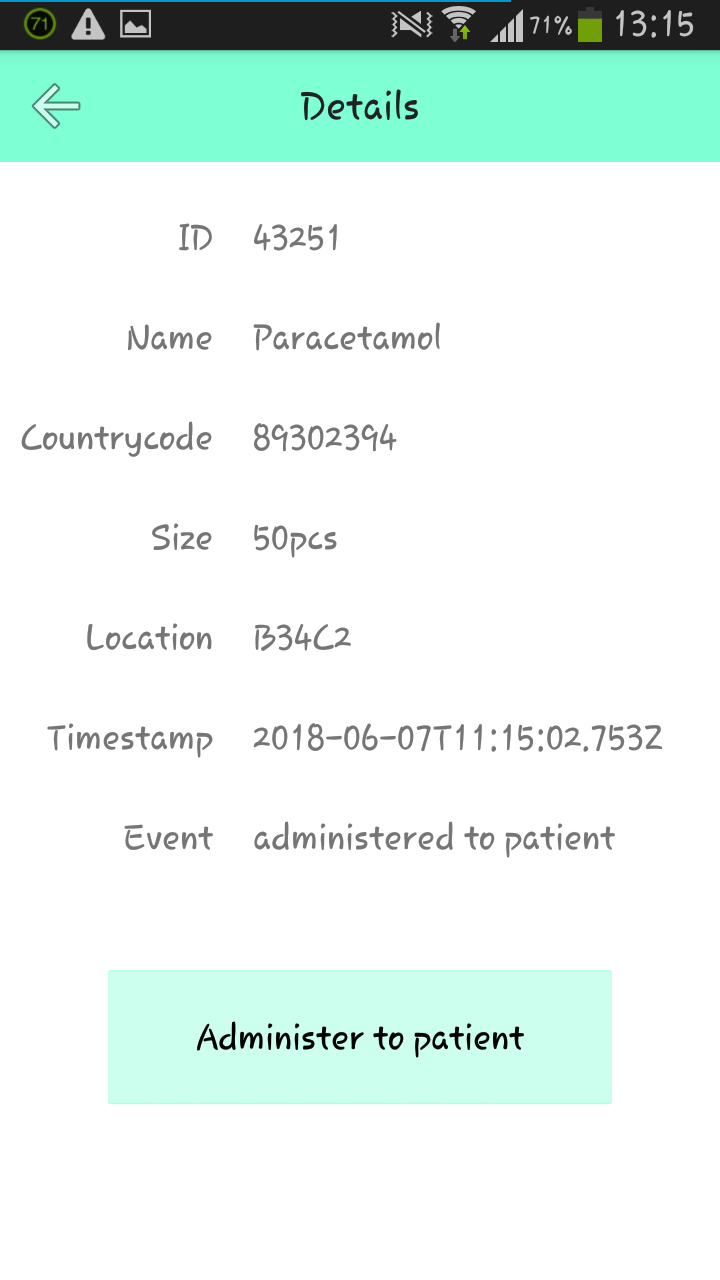
\includegraphics[width=4cm, height=8cm]{s3_03}}
\subfigure{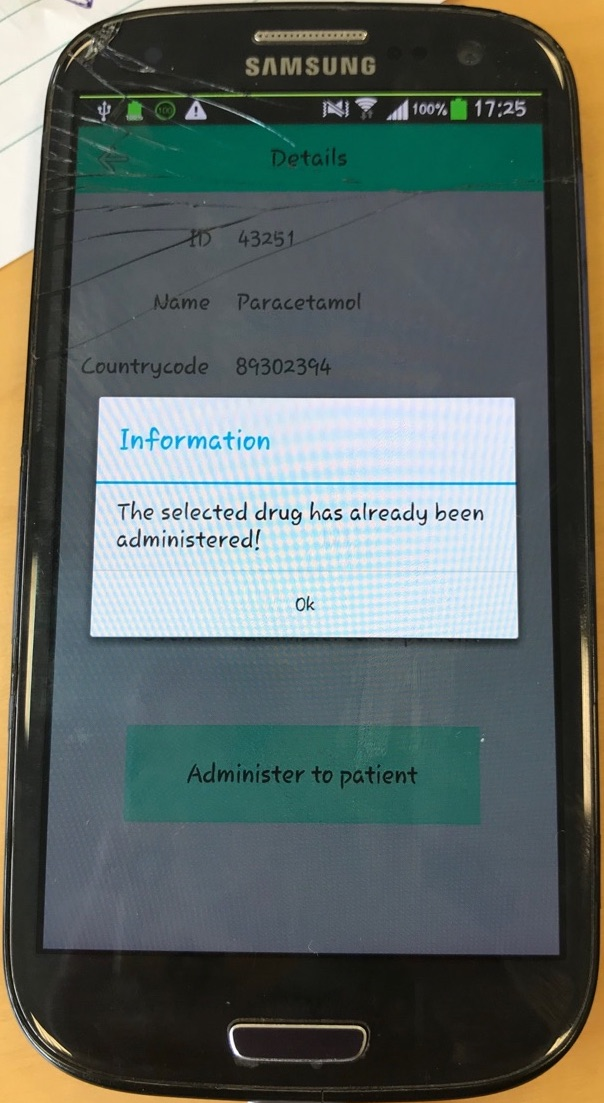
\includegraphics[width=4cm, height=8cm]{s3_04}}
\subfigure{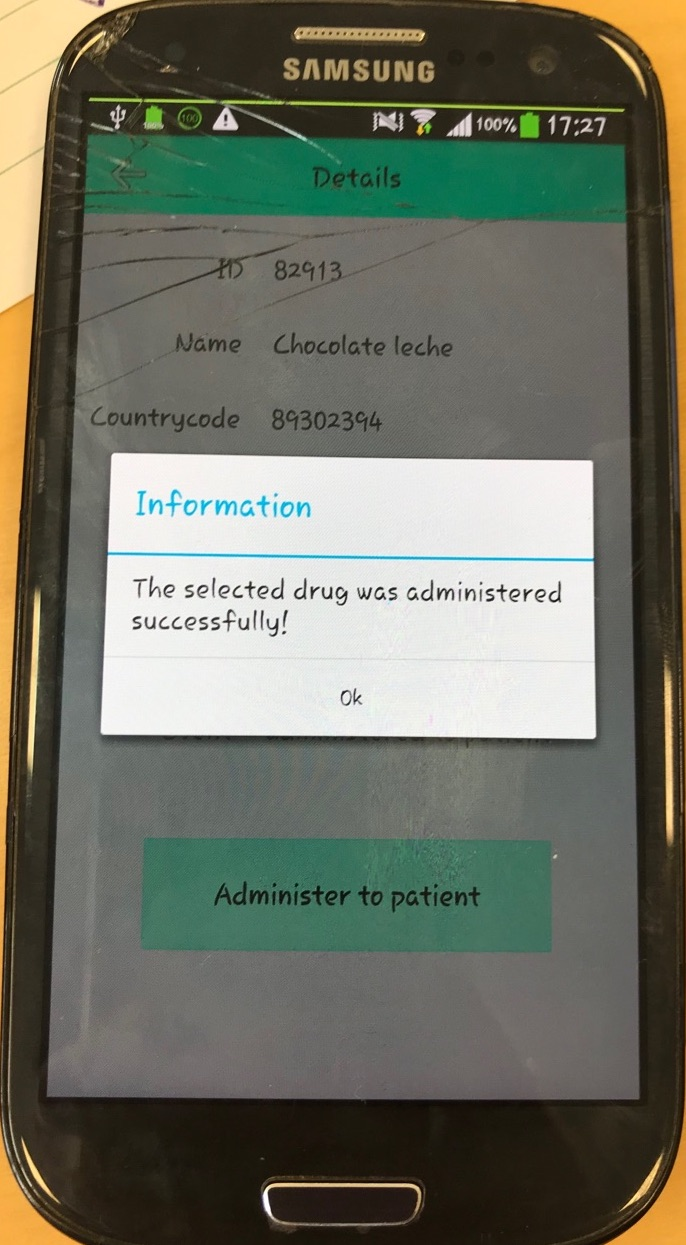
\includegraphics[width=4cm, height=8cm]{s3_05}}
\subfigure{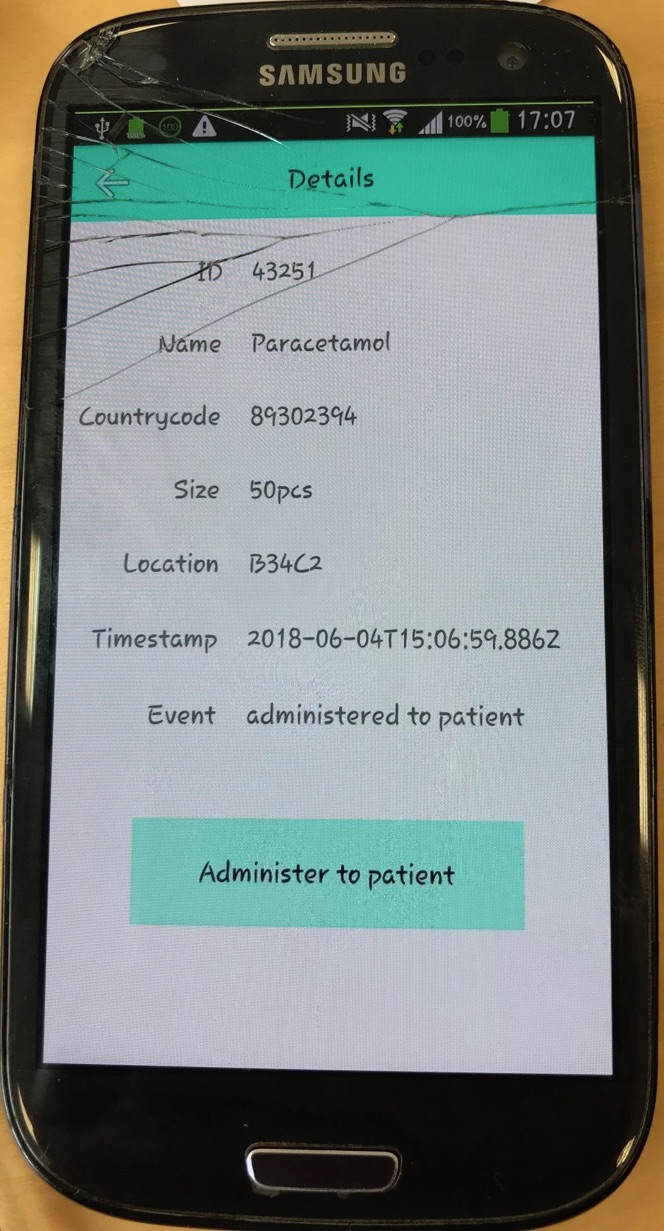
\includegraphics[width=4cm, height=8cm]{s3_06}}
\subfigure{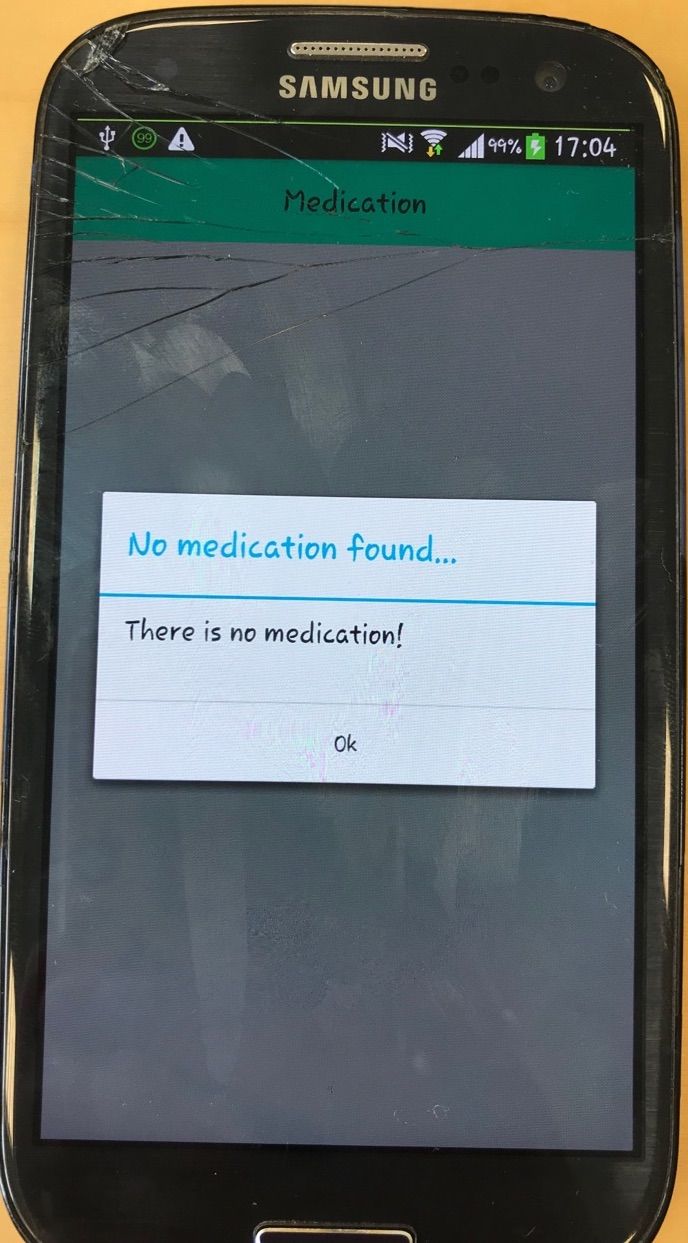
\includegraphics[width=4cm, height=8cm]{s3_07}}
\caption{\label{fig:s3_screenshots}Layout of application, Screenshot of iOS Simulator}
\end{figure}

successfull device tests: Samsung S3 GT I9300 (smartphone) see figure \ref{fig:s3_screenshots}

\subsection{Test results}

\subsection{Evaluation of test results}

\section{Summary and Outlook of application}

which are the problems when employing the system? 
costs of RFID, size of RFID...

\subsubsection{Extension possibilities}

Henrici \cite[p.121 ff.]{henrici} describes four alternative channels to authenticate and authorized the right tags and to prevent attacks on RFID applications. 
The first possibility of an alternative channel is to use written text to authenticate special operations, for instance on packaging. The master key can be printed on the interior of the product package and is proposed as key recovery mechanism.

Furthermore, optical barcodes can be used together with RFID to ensure identification of items. Especially barcodes attached to each item can be used for general identification of objects. Additionally, RFID tags might be used to assign items of high value.

A third possibility of using side channels is to use optical input, such as photodiodes attached to RFID tags. Each RFID tag can use flashes of light (also called optical channel) to transfer data.   
Lastly, a physical contact channel can also be used alternatively. Compared to smartcards, this methods defends against wireless sabotage or denial of service attacks.



\cleardoublepage
%\addcontentsline{toc}{chapter}{Bibliografía} %para añadir la bibliografía al indice

%\begin{thebibliography}{99}
\thispagestyle{fancy}
\printbibliography
%\end{thebibliography}
%%%%%%%%%%%%%%%%%%%%%%%%%%%%%%%%%%%%%%%%%%%%%%%%%%%%%%%%%%%%%%%%%%%%%%%%%%%%%%%%%%%%%%%%%%%%%%%%%%%%%%%%%%%%%%%%%%%%%%%%%%%%%%%%%%%%%%%%%%%%%%%%%%%%%%%%%%%
\let\cleardoublepage\clearpage
\clearpage

\ClearShipoutPicture


\appendix
\thispagestyle{fancy} %para que incluya las cabeceras y los pies de págnina en la primera página del capítulo (por defecto no lo pone) \label{cha:appendixA}
\chapter{\textbf{Abbreviations}}
% Die längste Abkürzung kann in die eckigen Klammern
% bei \begin{acronym} geschrieben, um einen häßlichen
% Umbruch zu verhindern
\begin{acronym}[WORM]
\acro{RFID}{Radio Frequency Identification}
\acro{NFC}{Near Field Communication}
\acro{IoT}{Internet of Things}
\acro{CT}{Computer Tomograph}
\acro{RTI}{Reusable Transport Items}
\acro{IT}{Information Technology}
\acro{UHF}{Ultra High Frequency}
\acro{RAIN}{RAdio Frequency IdentificatioN}
\acro{HIS}{Hospital Information System}
\acro{RIS}{Radiology Information System}
\acro{LIS}{Laboratory Information System}
\acro{EPC}{Electronic Product Code}
\acro{WORM}{Write Once Read Many}
\acro{WARD}{Wisely Aware RFID Dosage}
\acro{MIMS}{Mobile Intelligent Medical System}
\acro{LF}{Low Frequency}
\acro{HF}{High Frequency}
\acro{UHF}{Ultra High Frequency}
\acro{SSL}{Secure Sockets Layer}
\acro{TLS}{Transport Layer Security}
\acro{FDA}{Federal Drug Administration}
\acro{SMLE}{Single Logical Message Exchange}
\acro{SARS}{Severe Acute Respiratory Syndrome}
\acro{LBMS}{Location-based Medical Service}
\acro{TMUH}{Taipei Medical University Hospital}
\acro{ERP}{Enterprise Resource Planning}
\acro{HL7}{Health Level 7}
\acro{DICOM}{Digital Imaging and Communications in Medicine}
\acro{IoT}{Internet of Things}
\acro{CATS}{Compact Approximator based Tag Searching protocol}
\acro{ITSP}{Iterative Tag Search Protocol}
\acro{CW}{Continuous Wave}
\acro{VHF}{Very High Frequency}
\acro{RCS}{Radio Communication System}
\acro{UWB}{Ultra Wide-Band}
\acro{FMCW}{Frequency-Modulated Continuous Wave}
\acro{SNR}{signal-to-noise}
\acro{TDR}{time-domain reflectometry-based}
\acro{SAW}{surface acoustic wave}
\acro{CMT}{characteristic mode theory}
\acro{SEM}{singularity expansion method}
\acro{TOA}{time of arrival}
\acro{MF}{matched filter}
\acro{SOA}{Service-oriented architecture}
\acro{WLAN}{wireless local area network}
\acro{IrDA}{Infrared Data Association}
\acro{PC}{Personal Computer}
\acro{SOAP}{Simple Object Access Protocol}
\acro{API}{Application's Programming Interface}
\acro{WfMS}{Workflow-Management System}
\acro{ASP}{application-service-provider}
\acro{ESB}{Enterprise Service Bus}
\acro{SWOT}{Strengths Weaknesses Opportunities Threats}
\acro{CEP}{Complex Event Processing}
\acro{SME}{Small and Medium-sized enterprises}
\end{acronym}

\end{document}